%=========================================================================
% Autor: Jakub Duda 2022
\chapter{Úvod}
Myslím si, že nie je prehnané, keď poviem, že v~dnešnej dobe každý bežný človek prichádza do styku s~mapou celkom pravidelne. Väčšina ľudí si pri prvotnom zamyslení spojí mapy s~navigáciou a~orientáciou v~teréne. To je však len jedno z~mnohých využití máp. S~rôznymi typmi máp sa stretávame už od detstva. Či sa jedná o~mapu k~pokladu na nočnej hre v~tábore, mapu hydrosféry Slovenska v~učebnici geografie, mapu cestnej infraštruktúry v~televíznych novinách alebo cyklistickú mapu okolia na dovolenke v~Holandsku, všetko sú to špeciálne typy máp s~konkrétnym zameraním na isté prvky a~iné prvky zase vynechávajú. Pre takéto mapy bol pre účely tejto práce zavedený pojem \textbf{viac-menej slepé mapy}. Už z~krátkeho vymenovania použití viac-menej slepých máp je zrejmé, že škála ich uplatnenia je široká. Medzi najvýraznejšie sféry patrí vzdelávacia a~informačná, no tieto mapy nájdu uplatnenie aj v~mnohých menších a~viac špecifických odvetviach, ktoré pracujú s~istými prvkami geografického priestoru.

Na internete človek nájde množstvo mapových služieb, ktoré ponúkajú výborné všeobecné mapy. Menej sa už však nájde takých, ktoré ponúkajú aj mapy s~rôznym konkrétnym zameraním. Ak nejaké ponúkajú, tak je to väčšinou maximálne mapa s~čiernobielym podkladom, satelitná mapa alebo možno turistická či cyklistická mapa. Tam to však končí. Je to síce istá voľba zobrazených prvkov, no používateľa obmedzuje na niekoľko limitovaných možností. Lenže čo viac sa dá chcieť? Viac-menej slepé mapy sú totiž účelné mapy, ktoré sa zameriavajú na konkrétne odvetvia a~zobrazujú rôzne kombinácie prvkov. Takýchto kombinácií môžu byť stovky a je teda nemožné ponúkať také typy máp, ktoré by vyhoveli každému. 

Pri tvorbe viac-menej slepých máp je kľúčová možnosť voľby prvkov a~taktiež voľba ich dôležitosti a~výraznosti. Toto je predpoklad, ktorý musí spĺňať každý softvér určený na tvorbu a~generovanie takýchto máp a~práve takéto nástroje sú predmetom skúmania tejto práce. V~kapitole~\ref{theory} sa v~skratke venujem základom tvorby mapy, v~kapitolách~\ref{existing} a~\ref{tools} sa pozriem na funkčné existujúce riešenia, resp. dostupné nástroje, pomocou ktorých je takéto riešenie možné dosiahnuť. Kapitola~\ref{implementation} už potom opisuje moje vlastné riešenie tohto problému. 

Mojim riešením je webová aplikácia napísaná v~jazyku Python s~využitím frameworku Flask, ktorá pracuje s~dátami získanými z~projektu OpenStreetMap a~uloženými v~databáze s~geo-priestorovým rozšírením PostGIS. Stadiaľ sú dáta načítavané a~pomocou knižnice Mapnik, ktorá na tieto dáta aplikuje štýlové pravidlá definované pomocou súborov typu XML, je vygenerovaný výstupný súbor obsahujúci vytvorenú mapu. Obsah súbora je zo servera odoslaný klientovi, ktorý používateľovi umožní mapu stiahnuť. Aplikácia umožňuje tvorbu viac-menej slepých máp s~použitím preddefinovanej šablóny alebo s~použitím vlastnej štýlovej sady, ktorú je možné pomocou aplikácie vytvoriť. Aplikácia podporuje aj vloženie súborov typu GPX obsahujúcich trasy, ktoré vie vykresliť do mapy. Aplikácia taktiež obsahuje samostatnú sekciu dedikovanú úplne slepým mapám.

V kapitolách~\ref{idea} a~\ref{testing} je priblížený postup vzniku aplikácie a~to popisom návrhu a~analýzy požiadaviek, resp. popisom testovania aplikácie.  



\chapter{Problematika tvorby mapy}
\label{theory}
Táto kapitola sa venuje základným problémom, ktoré súvisia s~tvorbou a~tlačou máp. Hlavným zdrojom informácií v~podkapitole Kartografia~\ref{cartography} je internetový zdroj~\cite{cartography_3} a~potom~\cite{cartography_1} a~\cite{cartography_2}. V~podkapitole~\ref{print} sú informácie čerpané z~online článkov~\cite{printing_1} a~\cite{printing_2}.

\section{Kartografia}
\label{cartography}
Kartografia je vedný odbor, ktorá sa zaoberá tvorbou a~spracovaním máp. Často však býva označovaný aj ako technický a~umelecký odbor, čo pramení z~povahy problémov, ktorými sa zaoberá. História kartografie sa datuje až do obdobia niekoľkých stoviek rokov pred začiatkom nášho letopočtu, kedy vznikali prvé známe mapové diela. V~dnešnej dobe je proces tvorby máp značne zjednodušený existenciou rôznych softvérových doplnkov a~nástrojov. Čo sa však ani za stovky, či tisícky rokov nezmenilo sú ciele kartografie. Cieľom každého kartografického diela je čo najlepšie naplnenie piatich základných aspektov:
\begin{itemize}
  \item{\bf presnosť \rm - úroveň presnosti s~akou mapa korešponduje s~reálnym svetom}
  \item{\bf funkcionalita \rm - schopnosť mapy plniť svoju funkciu, prezentovať informáciu}
  \item{\bf jednoznačnosť \rm - úroveň jednoduchosti s~akou plní mapa svoju funkciu a~poskytuje žiadanú informáciu}
  \item{\bf bohatosť \rm - úroveň rozmanitosti poskytnutej informácie}
  \item{\bf estetický dojem \rm - emocionálna reakcia na mapu ako celok}
\end{itemize}
Tieto aspekty však často idú proti sebe a~priorizovaním jedného z~nich, sú zase zanedbávané ostatné, čo znižuje kvalitu výsledného diela. Cieľom preto je nájsť čo najlepší kompromis. Na dosiahnutie tohto cieľa musí kartografia vyriešiť šesť hlavných problémov:
\begin{itemize}
  \item{dáta a~generalizácia}
  \item{projekcia}
  \item{symbolika}
  \item{typografia}
  \item{kompozícia mapy}
  \item{rozloženie mapy}
\end{itemize}

\subsection*{Dáta a~generalizácia}
Prvou zastávkou v~procese tvorby máp sú dáta. Aby vôbec bolo možné niečo na mape zobraziť je potreba mať k~dispozícií dáta, ktoré popisujú prvky reálneho sveta. V~dnešnej dobe existuje obrovské množstvo dostupných geografických dát. Pri tvorbe mapy však treba dbať ohľad na vhodnosť dát, nie všetky dáta sú totiž vhodné pre každý typ a~mierku mapy. Dôležitým parametrom pri výbere dát je ich zložitosť. Komplexnosť reálneho sveta je totiž nekonečná a~vie byť zaznamenaná len do istej miery. No a~na mape je toho možné zobraziť ešte menej. Kartograf preto musí pri tvorbe mapy zvoliť dáta s~vhodnou úrovňou detailu. Tento proces sa nazýva generalizácia, resp. zovšeobecňovanie a~spočíva v~strategickom výbere prvkov, ktoré dáva zmysel vykresliť pri danom type a~danej mierke mapy.

\subsection*{Projekcia}
Keďže Zem má tvar gule, presnejšie elipsoidu, kartograf musí vyriešiť problém akým spôsobom zobraziť zemský povrch na dvojrozmernej mape. Zobrazenie zemského povrchu do roviny sa nazýva projekcia a~spočíva v~aplikovaní algoritmov, pomocou ktorých sú súradnice skutočného zemského povrchu transformované do súradníc roviny. Aby však niečo takéto bolo dosiahnuteľné, z~princípu musí vznikať \bf skreslenie\rm. Nie je možné zároveň zachovať tvar objektov, vzdialenosť medzi nimi a~aj uhly, ktoré zvierajú. Záležiac od typu mapy sú niektoré druhy skreslenia akceptovateľné, ale iné zase nie, a~preto existuje množstvo rôznych projekcií, resp. zobrazení, ktoré sa zameriavajú na zachovanie rôznych vlastností zemského povrchu. Na základe toho, ktoré vlastnosti sú zachované, sa projekcie rozdeľujú na:
\begin{itemize}
  \item{\bf ekvidistančné \rm - zachovávajú vzdialenosti v~určitom smere}
  \item{\bf ekvivalentné \rm - zachovávajú pomery plôch, ale výrazne skresľujú uhly}
  \item{\bf konformné \rm - zachovávajú uhly, ale výrazne skresľujú plochy}
  \item{\bf vyrovnávajúce, resp. kompromisné \rm - skreslenie uhlov a~plôch v~malej miere so snahou nájsť kompromis}
\end{itemize}
Projekcie sa tiež líšia v~druhu telesa, na ktoré je zemský povrch zobrazený. 

\begin{figure}[hbt]
	\centering
	\includegraphics[width=0.6\textwidth]{obrazky-figures/mercator.pdf}
	\caption{Obrázok zemského povrchu zobrazeného pomocou Mercatorovho zobrazenia, ktorý využíva Tissotovú indikatrix na demonštráciu skreslenia veľkosti území. Vykreslené oranžové body reprezentujú územia, ktoré sú v~skutočnosti rovnako veľké. Obrázok je prevzatý z~\cite{mercator} pod licenciou\protect\footnotemark}
	\label{img_mercator}
\end{figure}

Najznámejším a~najčastejšie používaným zobrazením je \bf Mercatorovo zobrazenie\rm, ktoré zobrazuje zemský povrch na valec. Toto zobrazenie je konformným zobrazením, ktoré zachováva tvary telies, uhly medzi nimi a~tiež smer. Jeho výhodou je, že zachováva orientáciu na sever, vďaka čomu sa stalo štandardom pri navigácii. Najväčšou nevýhodou tohoto zobrazenia je, že výrazne skresľuje veľkosť území, ktoré sa nachádzajú vo veľkej vzdialenosti od rovníka, čo je možné pozorovať na obrázku~\ref{img_mercator}. Napríklad územie celej Afriky a~územie Grónska, ktoré je v~skutočnosti štrnásťkrát menšie, sa pri zobrazení celého sveta pomocou Mercatorovho zobrazenia javia ako rovnako veľké. Aj napriek jeho nevýhodám je však toto zobrazenie v~kompromisnom variante nazývanom {\it Web Mercator} používané v~takmer všetkých popredných mapových službách ako Google Maps, OpenStreetMap, MapBox či MapQuest.

Pre územie Českej republiky a~Slovenska je tiež zaujímavé tzv. \bf Křovákovo zobrazenie\rm, vytvorené Josefom Krovákom v~roku 1922. Toto zobrazenie na rozdiel od Mercatorovho, zemský povrch zobrazuje na kužeľ. Je konformné a~ekvidistančné. Křovákovo zobrazenie bolo optimalizované pre územie Česka a~Slovenska a~je najpresnejším zobrazením tohoto územia. Jeho nevýhodou je pootočenie v~kladnom smere, ktoré skresľuje vzájomnú polohu jednotlivých častí krajín. Variant tohoto zobrazenia nazývaný {\it Systém jednotné trigonometrické sítě katastrální} je používaný v~geodézií v~Českej republike a~na Slovensku. Porovnanie s~Mercatorovým zobrazením je ukázané na obrázku~\ref{img_krovak}.

\footnotetext{Creative Commons Attribution-Share Alike 4.0 International License, \url{https://creativecommons.org/licenses/by-sa/4.0/deed.en}}

\begin{figure}[hbt]
	\centering
	\includegraphics[width=0.5\textwidth]{obrazky-figures/img_krovak_cz.pdf}\hfill
	\includegraphics[width=0.5\textwidth]{obrazky-figures/img_merc_cz.pdf}\hfill
	\caption{Obrázok porovnávajúci zobrazenie územia Českej republiky v~Křovákovom (vľavo) a~Mercatorovom (vpravo) zobrazení.}
	\label{img_krovak}
\end{figure}


\subsection*{Typografia}
Dôležitou súčasťou mapy je text. Text slúži na identifikovanie prvkov mapy podľa názvu, ale tiež sa podieľa na tvorbe vizuálnej hierarchie mapy a~jej estetického dojmu. Text na mape musí spĺňať dve základné pravidlá, a~to čitateľnosť a~zrejmú príslušnosť ku konkrétnemu prvku mapy. Na dosiahnutie týchto cieľov musí kartograf pre textový popis každého prvku vybrať vhodné parametre. 

Najzákladnejším parametrom je \bf typ písma\rm. Pri voľbe typu písma je dôležité zvážiť niekoľko vlastností. Zvolený typ musí byť čitateľný aj pri malých veľkostiach, jednotlivé písmená musia byť od seba jednoducho rozlíšiteľné a~viditeľne odlišné musia byť aj rôzne fonty tohto typu písma ako napríklad tučné písmo alebo kurzíva. Nepísaným pravidlom je voľba jedného, nanajvýš dvoch rôznych typov písma.~\cite{typography}

Medzi ďalšie dôležité parametre patrí farba, veľkosť, orientácia, hrúbka písma, obrys písma, vzdialenosť písmen, riadkovanie a~zalamovanie do riadkov. V~neposlednom rade je potrebné správne vybrať, ktoré prvky vôbec budú textom označené, a~ktoré nie, aby nebola narušená prehľadnosť mapy. Na obrázku~\ref{img_typography} je možne pozorovať porovnanie máp, ktoré sa líšia len voľbou vhodných typografických parametrov.

\begin{figure}[hbt]
	\centering
	\includegraphics[width=1\textwidth]{obrazky-figures/bad_typography.pdf}\hfill
	\includegraphics[width=1\textwidth]{obrazky-figures/good_typography.pdf}\hfill
	\caption{Obrázok porovnávajúci mapu bez nastavenia typografických parametrov (hore) a~mapu so zvolenými vhodnými typografickými parametrami (dole). Prehľadnosť prvej mapy je omnoho nižšia a~je do istej úrovne zachovaná len vďaka využitiu symboliky. Druhá mapa pomocou nastavenia farby naznačuje príslušnosť textu k~prvkom, voľbou veľkosti zdôrazňuje dôležitosť prvku a~k prehľadnosti prispieva zahrnutím len vhodného počtu textových informácií. Mapy sú vygenerované pomocou vytvorenej aplikácie.}
	\label{img_typography}
\end{figure}

\subsection*{Symbolika}
Úlohou symboliky na mape je podať informáciu používateľovi, čo najefektívnejšie. Mapy sú totiž len zmenšeninou zemského povrchu, z~čoho vyplýva, že kartograf pracuje s~limitovaným priestorom a~nie je možné označiť každý prvok textom. Takéto označenie by navyše bolo veľmi neprehľadné a~z toho dôvodu sa pri tvorbe mapy musí využívať symbolika. Symbolika neoznačuje len použitie symbolov -- piktogramov, ale spôsob vizuálneho zobrazenia každého jedného z~prvkov mapy. 

Vytvorenie mapového symbolu, ktorým je reprezentovaný prvok mapy spočíva v~zvolení správnych hodnôt parametrov, ktoré určujú jeho vzhľad. Voľbou rôznych hodnôt sa kartograf snaží zabezpečiť kontrast medzi rôznymi prvkami a~vrstvami mapy, vizuálnu hierarchiu prvkov a~tiež dobrý celkový estetický dojem mapy. Medzi najčastejšie využívané parametre patrí veľkosť, tvar, orientácia, farba, sýtosť, priehľadnosť alebo použitie vzoru. Voľba symboliky prvku vychádza z~jeho vlastností, najmä dimenzie a~dôležitosti. Na základe dimenzie je možné prvky mapy rozdeliť do troch kategórií: \bf body\rm, \bf línie \rm a~\bf mnohouholníky\rm. Prvky každej z~týchto kategórií využívajú iné symbolické parametre. 

\bf Symbolika mnohouholníkov \rm najčastejšie využíva voľba tvaru, farby, priehľadnosti, farby obrysu alebo použite vzoru. Mnohouholníky sú najčastejšie vykreslené ako geometrické útvary s~farebnou výplňou. Voľba farby je väčšinou spojená so snahou o~pripodobnenie k~reálnemu svetu, ako napríklad použitie tmavšej zelenej pre lesné porasty a~svetlejšej pre trávnaté územia. Nastavenie priehľadnosti môže byť využité na vyjadrenie dôležitosti prvku alebo na zníženie zásahu do zobrazenia menších prvkov nachádzajúcich sa vo vnútri mnohouholníka. Použitím vzoru je možné zvýrazniť a~tiež odlíšiť zvolený prvok. Mnohouholníky, ktoré nereprezentujú skutočné územia zemského povrchu, ale len pomyselné územia definované človekom, ako napríklad administratívne celky, často bývajú symbolizované len svojim obrysom, aby nenarušovali vykreslenie menších prvkov. Malé mnohouholníky zase môžu byť symbolizované pomocou použitia piktogramu, podobne ako body. Pri vykreslení mnohouholníkov je tiež dôležité dbať na poradie, aby sa nestalo, že väčšie mnohouholníky prekryjú menšie, ktoré môžu mať vyššiu dôležitosť.

Pri \bf symbolike línií \rm je najdôležitejšia voľba veľkosti -- hrúbky a~farby, ktoré reprezentujú dôležitosť a~typ prvku. Na vyjadrenie jemnej odlišnosti prvkov, ako napríklad odlíšenie tunelu od bežnej cesty, sa často používa nastavenie ďalších parametrov ako obrys, priehľadnosť, či tvorba prerušovaných línií. Pri tvorbe symboliky línií je dôležité zachovanie zaužívaných farieb pre rôzne často zobrazované prvky, ako napríklad použitie červenej farby na vykreslenie diaľnic.

Najzložitejšia je \bf symbolika bodov\rm. Body sú najmenším typom prvku a~na vytvorenie ich symbolu a~prezentovanie informácie je na mape dostupný najmenší priestor. Ako symboly bodov sa využívajú piktogramy, ktoré musia tieto body jednoznačne identifikovať. Symboly väčšinou využívajú zjednodušenú reprezentáciu skutočnej podoby prvku alebo podoby nejakého objektu, ktorý prvok jednoznačne reprezentuje. Príkladom je piktogram príboru reprezentujúci reštauráciu, alebo piktogram kotvy reprezentujúci prístav. Dôležitým faktorom je tiež zvolenie farby, ktorá môže slúžiť na rozlíšenie rôznych prvkov a~vytváranie tematických skupín prvkov.

\subsection*{Kompozícia mapy}
Kompozícia mapy opisuje vykreslenie jednotlivých prvkov mapy ako celku. Jednotlivé symboly a~popisy môžu byť dobre nadizajnované, no môže sa stať, že mapa aj napriek tomu nevyzerá dobre. Všetky prvky mapy musia byť totiž dobre nadizajnované ako celok, čo znamená, že prvky nesmú byť navzájom rušivé a~naopak musia vytvárať \uv{symbiózu}, ktorá vedie k~jednoznačnosti a~prehľadnosti mapy. Pri riešení problému kompozície mapy sa musí kartograf zaoberať zvolením správnych symbolov tak, aby boli jednoducho separovateľné od podkladu mapy a~tiež od symbolov označujúcich prvky iného typu. Takisto musí dbať na to, aby bola na základe zvolených symbolov zrejmá dôležitosť prvkov mapy.

\subsection*{Rozloženie mapy}
Rozložením mapy je označené rozmiestnenie celkového produktu tvorby mapy, zahŕňajúceho nielen samotnú mapu, ale aj sprievodné prvky mapy, medzi ktoré patrí napríklad názov, legenda, vyznačenie mierky a~orientácie mapy, doplňujúci text a~ilustrácie, či metadáta mapy. Tieto prvky slúžia na doplnenie informácie, ktorá nie je zo samotnej mapy úplne zrejmá a~používateľovi by mohla chýbať, čo by znamenalo, že mapa neplní svoju funkciu. Zahrnutie sprievodných prvkov závisí od typu mapy a~jej účelu a~napríklad pri generovaní viac-menej slepých máp na osobné účely, ktorých prvky si navolil sám používateľ, a~teda k~nim nepotrebuje žiadnu vysvetľujúcu informáciu, nie je nutné.


\section{Tlač máp}
\label{print}
 Pri zameraní tvorby mapy na tlač sa objavuje nová premenná, ktorá zohráva rolu vo výslednej kvalite mapy. Je to premenná, ktorá sa nazýva \bf DPI\rm\footnote{\bf DPI \rm (Dots per inch) -- počet bodov na palec}. Táto hodnota vyjadruje koľko skutočných bodov bude vytlačených na jeden palec papiera, čiže 2,54 cm. Súvisiacou premennou je hodnota \bf PPI\rm\footnote{\bf PPI \rm (Pixels per inch) -- počet pixelov na palec}. Ohľadom týchto dvoch premenných často vznikajú nedorozumenia, no v~skutočnosti sú prakticky zameniteľné. Kým DPI vyjadruje počet bodov na papieri, PPI vyjadruje počet pixelov na obrazovke. Nastavenie PPI, či DPI obrázka alebo mapy je mierne abstraktným pojmom. Niektoré softvéry slúžiace na editovanie obrázkov toto nastavenie poskytujú, no v~skutočnosti sa jedná len o~vytvorenie záznamu v~metadátach obrázku, ktorý slúži ako informácia pre tlačiareň, s~využitím akého DPI má byť obrázok alebo mapa vytlačená. Pri tvorbe digitálnych máp teda na PPI, resp. DPI vôbec nezáleží a~dôležité je len pri tlači. 

Hodnota DPI je určená fyzickou špecifikáciou tlačiarne a~na moderných tlačiarňach môže byť nastavovateľná. Čím je použitá hodnota DPI vyššia, tým ostrejšia a~kvalitnejšia bude vytlačená mapa. Vyžadovaným štandardom pre kvalitnú tlač je 300 DPI. Hodnoty nižšie ako 200 DPI sa pri tlači považujú za nedostatočné. Keď má teda používateľ záujem vytlačiť mapu so šírkou 254 centimetrov, čo činí 100 palcov a~používa nastavenie 300 DPI, musí zabezpečiť aby súbor, ktorý obsahuje mapu mal na šírku 100 * 300 = 30 000 pixelov. Pri použití 600 DPI by to bolo 60 000 pixelov.

Problém voľby DPI a~generovania máp so správnym rozmerom je však veľmi jednoducho eliminovateľný, a~to zmenou výstupného formátu z~rastrového na vektorový. Kým rastrové súbory sú tvorené z~pixelov a~pri zmene veľkosti strácajú na kvalite, vektorové súbory sú definované pomocou objektov a~pred tlačou teda môžu byť ľubovoľne zväčšované alebo zmenšované bez akejkoľvek straty kvality.


\chapter{Existujúce nástroje na generovanie viac-menej slepých máp}
Táto kapitola sa zaoberá skúmaním dostupných nástrojov na tvorbu viac-menej slepých máp. Zameriava sa na ich možnosti a~použitie.

\label{existing}
\section{Webové mapové služby}
Exsituje množstvo rôznych webových služieb, ktoré sú zamerané na poskytovanie máp. Medzi najrozšírenejšie patria napríklad Google Maps, OpenStreetMap alebo na území Česka a~Slovenska služba Mapy.cz. Služba OpenStreetMap je rozsiahlym projektom, ktorému je venovaná samostatná kapitola~\ref{osm}. Okrem iného ponúka mapového klienta slúžiaceho na prehliadanie máp. Tento klient podobne ako služba Mapy.cz fungujú na princípe tzv. rastrových dlaždíc, čo sú rastrové obrázky uložené na serveri, ktoré sú na základe požiadavkov odosielané klientovi, kde sú v~prehliadači pospájané do výslednej mapy. Tieto služby síce ponúkajú možnosť stiahnutia mapy pre tlač, no ponúkajú však len niekoľko preddefinovaných typov mapy bez možnosti selekcie prvkov a~ich zobrazenia. Toto samozrejme súvisí s~využitím technológie rastrových dlaždíc.

\subsection*{mapstyle.withgoogle.com}
Služba Google Maps je založená na princípe vektorových dlaždíc. Princíp vektorových dlaždíc je podobný ako pri rastrových dlaždiciach, ale líši sa v~tom, že časti mapy sú používateľovi dodávané vo vektorových súboroch. Keďže vektorové súbory sú tvorené definíciami objektov, je vcelku jednoduché meniť rôzne parametre, ktoré definujú vykreslenie objektov -- prvkov mapy. Na tomto princípe funguje zaujímavý nástroj {\it mapstyle.withgoogle.com}\footnote{\url{https://mapstyle.withgoogle.com/}}. Tento nástroj umožňuje zmenu základných symbolických parametrov pre vyše tridsať skupín objektov mapy. Medzi nastaviteľnými parametrami sú napríklad farba, sýtosť a~hrúbka, ktoré je možné nastaviť pre výplň, čiary či text. Pre jednotlivé skupiny prvkov je tiež možné nastaviť, či sú zobrazené alebo nie. Nevýhodou nástroja je slabšia voľnosť pri definícií zobrazenia konkrétnych prvkov, nakoľko ich zobrazenie závisí od skupiny, do ktorej sú zaradené a~je možné nastavovať parametre len pre celú skupinu. Snímka užívateľského rozhrania tohto nástroja je na obrázku~\ref{img_google}

\begin{figure}[hbt]
	\centering
	\includegraphics[width=0.8\textwidth]{obrazky-figures/img_google.png}
	\caption{Obrázok zobrazujúci užívateľské rozhranie nástroja {\it mapstyle.withgoogle.com}. Na ľavej strane rozhrania sa nachádza ovládací panel obsahujúci nastavovateľné prvky. Po rozkliknutí prvku sa panel rozšíri a~zobrazia sa možnosti editovania zobrazenia prvku.}
	\label{img_google}
\end{figure}

\section{Aplikácie}
GIS alebo geografický informačný systém je informačný systém slúžiaci na tvorbu, správu, analýzu a~vizualizáciu geo-priestorových dát. Geo-priestorovými dátami sa rozumejú dáta, ktoré vyznačujú alebo súvisia s~konkrétnou geografickou polohou. Geografický informačný systém sa spravidla skladá z~databázy a~softvérových nástrojov umožňujúcich vykonávanie spomenutých operácií. Často takto však bývajú označované aj rôzne softvérové nástroje orientované na geo-priestorové dáta a~prácu s~nimi.

Medzi najznámejšie geografické informačné systémy patrí ArcGIS, QGIS alebo Maptitude. ArcGIS\footnote{\url{https://www.arcgis.com/index.html}} aj Maptitude\footnote{\url{https://www.caliper.com/maptovu.htm}} sú komerčné softvérové produkty. V~tejto podkapitole bude používateľ bližšie oboznámený s~voľne dostupným geografickým systémom QGIS~\ref{qgis} a~tiež aplikáciou Maperative~\ref{maperitive}.

\subsection*{QGIS}
\label{qgis}
QGIS\footnote{\url{https://qgis.org/en/site/}} je open-source softvér dostupný pre všetky bežné platformy ako Windows, Linux, Mac alebo Android. Napísaný je hlavne v~jazyku C++ s~využitím nástroja Qt. V~porovnaní s~ArcGIS ponúka menšie množstvo nástrojov, ktorých funkcionalitu je ale množné nahradiť použitím dostupných rozšírení. QGIS je schopný načítať dáta v~rôznych formátoch ako ESRI Shapefile\footnote{ESRI Shapefile -- formát obsahujúci geo-priestorové vektorové dáta.}, OSM formáty OSM XML a OSM PBF, popísané v kapitole~\ref{osm_format}, a~tiež umožňuje čítanie dát z~databázových systémov ako napríklad PostGIS. Podporuje tiež načítanie a~vektorizáciu rastrových súborov alebo import a~prácu s~GPS dátami v~súboroch typu GPX. Na obrázku~\ref{img_qgis_ui} je ukázané užívateľské rozhranie aplikácie.

V sekcií \uv{Style Library} ponúka QGIS rozsiahle nastavenia štýlu mapy. Nastavenie štýlov je rozdelené podľa typov prvkov na štýly zobrazenia bodov, línií, štýly výplní, štýl textu, štítkov a~rozsiahle nastavenia farby. Je možné importovať vlastné symboly alebo symboly získané z~online úložiska symbolov\footnote{\url{https://plugins.qgis.org/styles/}}. QGIS tiež podporuje tvorbu nových symbolov na princípe definovania základných tvarov a~ich skladania do stromovej štruktúry pomocou nastavenia v~užívateľskom rozhraní zobrazenom na obrázku~\ref{img_qgis_symbol}. Zaujímavá je aj možnosť tvorby línií, ktorých šírka a~farba sa mení pozdĺž línie. Podporované je aj použitie 3D symbolov.~\cite{qgis}


\begin{figure}[hbt]
	\centering
	\includegraphics[width=0.8\textwidth]{obrazky-figures/qgis.png}
	\caption{Obrázok zobrazujúci užívateľské rozhranie aplikácie QGIS. Číslo 1 označuje menu, 2 - panel nástrojov, 3 - rôzne panely s~možnosťami ako napríklad správa dátových zdrojov alebo selekcia vrstiev, 4 - zobrazenie mapy a~5 označuje statusový panel. Obrázok je prebratý z~oficiálnej dokumentácie. Obrázok prebratý z dokumentácie~\cite{qgis_img_1}.}
	\label{img_qgis_ui}
\end{figure}

\begin{figure}[hbt]
	\centering
	\includegraphics[width=0.5\textwidth]{obrazky-figures/qgis_symbol.png}
	\caption{Obrázok zobrazujúci možnosť vytvorenia nového symbolu v~aplikácií QGIS. Obrázok je prebratý z~oficiálnej dokumentácie. Obrázok prebratý z dokumentácie~\cite{qgis_img_2}.}
	\label{img_qgis_symbol}
\end{figure}

\subsection*{Maperitive}
\label{maperitive}
Maperitive\footnote{\url{http://maperitive.net/}} je zadarmo dostupná aplikácia dostupná pre Windows, Linux a~Mac napísaná v~jazyku C\#. Aplikácia umožňuje načítať dáta, aplikovať štýl a~exportovať vytvorenú mapu. Aplikácia primárne pracuje s~dátami OpenStreetMap a~podporuje tiež načítanie GPS dát. Nevýhodou je, že nepodporuje načítavanie dát z~databázy a~pre väčšie územia je tým pádom potrebná manipulácia s~veľkými exportmi dát z~OpenStreetMap. Maperitive dokáže generovať mapy vo formátoch BMP, PNG alebo SVG.

Na definovanie štýlu mapy sú používané špeciálne typy súborov nazývané \uv{ruleset}, teda súbor pravidiel. Maperitive umožňuje použitie jedného z~vstavaných súborov pravidiel ako OpenStretMap, Google Maps alebo Turistický súbor pravidiel. Špeciálnym súborom pravidiel je tzv. \uv{Wireframe ruleset}, ktorý veľmi jednoduchým štýlom vykresľuje všetky dostupné prvky a~slúži na identifikovanie ešte nepokrytých prvkov pri tvorbe vlastného štýlu. Tvorba vlastného štýlu sa skladá z~výberu vykreslených prvkov, nastavenia parametrov mapy a~definíciou pravidiel, ktoré určujú spôsob vykreslenie daných prvkov. Príklad súboru pravidiel je ukazáný v~kódovom výpise~\ref{maperitive_code}.

Výber prvkov je realizovaný na základe adresovania prvkov pomocou atribútov a~ich hodnôt. Je rozdelený podľa typu prvkov, a~teda na body, línie a~územia. Prvky sú vyberané do skupín s~názvom, na základe ktorého sú adresovateľné pri definícii pravidiel. Pri adresovaní je tiež možné využiť regulárne výrazy. 

Definícia pravidiel sa skladá z~výberu cieľa -- skupiny definovanej pri výbere prvkov -- a~následným definovaním rôznych parametrov ako farba, hrúbka a~množstvo ďalších. Pri definícií pravidiel je tiež možné použiť klasickú konštrukciu {\tt if-else} alebo kľúčové slovo {\tt for} slúžiace na definovanie podskupiny.~\cite{maperitive}

\begin{lstlisting}[frame=single,aboveskip=20pt,belowskip=20pt,framesep=10pt,caption={Príklad súboru pravidiel v~aplikácií Maperitive. Vyberá prvky typu bod označujúce zastávky električiek a~definuje ako majú byť vykreslené.},label={maperitive_code}]
features
    points
        tram stop : railway=tram_stop
rules
    target : tram stop
        define
            icon-image : symbols/tram_stop.png
\end{lstlisting}


\chapter{Dostupné technológie pre programové riešenie generovania viac-menej slepých máp}
\label{tools}
Táto kapitola popisuje rôzne technológie a~nástroje, ktoré môžu byť použité pri tvorbe viac-menej slepých máp. Technológie využité pri tvorbe aplikácie sú rozobraté podrobnejšie.

\section{OpenStreetMap}
\label{osm}
OpenStreetMap\footnote{\url{https://www.openstreetmap.org/}}, skrátene OSM je projekt, ktorého cieľom je vytvorenie voľne dostupnej databázy geografických dát celého sveta. Tento projekt vznikol s~účelom poskytovať geografické dáta, ktoré sú bez legálnych alebo technických obmedzení voľne dostupné pre kohokoľvek na akékoľvek produktívne alebo kreatívne využitie. Zbieranie dát je založené na voľnom prispievaní používateľov. OpenStreetMap okrem geografických dát ponúka aj mapového klienta a~množstvo rozhraní určených na prispievanie novými dátami. Informácie v tejto kapitole boli čerpané z~\cite{osm_page} a~\cite{osm_article}.

\subsection*{História}
Projekt OpenStreetMap založil Steve Coast vo Veľkej Británii v~roku 2004. Spočiatku bol projekt zameraný na vytvorenie dostupného zdroja dát pre územie Veľkej Británie. V~roku 2006 bola založená nadácia OpenStreetMap s~cieľom podporiť vznik a~šírenie geografických dát. V~roku 2006 bol tiež prvý krát spustený mapový klient. Projekt sa postupne rozrastal a~zlepšovali sa aj možnosti kontribúcie dát. V~roku 2008 bol počet registrovaných užívateľov približne 50 000 a~počet uzlov definujúcich geografické dáta v~databáze presahoval 300 miliónov. K~januáru 2022 zaznamenal OpenStreetMap 8,3 milióna registrovaných používateľov a~7,4 miliárd uzlov. V~poslednom kvartáli roku 2021 priemerný počet zmien za jeden deň činil približne 4 milióny. Na obrázku~\ref{img_osm_contrib} je zobrazený počet aktívnych používateľov za mesiac počas celej histórie projektu. Množstvo ďalších štatistík je dostupných na oficiálnej stránke.\footnote{\url{https://wiki.openstreetmap.org/wiki/Stats}}

\begin{figure}[hbt]
	\centering
	\includegraphics[width=0.8\textwidth]{obrazky-figures/osm_contributors.png}
	\caption{Obrázok zobrazujúci počet aktívnych prispievateľov dát do projektu OSM za mesiac počas celého obdobia existenice projektu. Obrázok prebratý z dokumentácie~\cite{osm_contributors} a upravený.}
	\label{img_osm_contrib}
\end{figure}


\subsection*{Využitie}
V dnešnej dobe sú dáta z~projektu OpenStreetMap využívané mnohými svetoznámymi spoločnosťami. Medzi najznámejšie spoločnosti, ktoré dáta z~OSM využívajú alebo využívali v~histórií patrí napríklad Amazon, Apple, Craigslist, Facebook, Snapchat, či Tesla. Medzi menej vysokoprofilové spoločnosti využívajúce dátové služby OSM patria napríklad spoločnosti vytvárajúce športovo orientované aplikácie ako Komoot\footnote{\url{https://www.komoot.com/}} alebo Strava\footnote{\url{https://www.strava.com/}}, či spoločnosti poskytujúce mapové služby ako Mapbox\footnote{\url{https://www.mapbox.com/}}, alebo Mapy.cz\footnote{\url{https://www.mapy.cz/}}. Na obrázku~\ref{img_strava} je zobrazený príklad mapy v~aplikácii Strava. 

\begin{figure}[hbt]
	\centering
	\includegraphics[width=0.6\textwidth]{obrazky-figures/img_strava.png}
	\caption{Snímok obrazovky zobrazujúci mapu v~aplikácii Strava. Aplikácia Strava je aplikácia zameraná na zaznamenávanie GPS údajov športových aktivít. Na snímku obrazovky je zobrazená mapa použitá pri zobrazení konkrétnej aktivity. V~pravom dolnom rohu je možné sledovať atribúciu mapy.}
	\label{img_strava}
\end{figure}

Väčšina spoločností využíva dáta OSM, na základe ktorých vytvárajú vlastné mapy, ktoré poskytujú, či už ako svoj primárny alebo len sprievodný produkt. Spoločnosti ako Amazon, Apple alebo Facebook sú však aktívne aj na druhej strane procesu tvorby geografickej databázy sveta. Spoločnosť Amazon, ktorá využíva dáta OSM na navigáciu pri procese doručovania zásielok, zbiera od používateľov spätnú väzbu, na základe ktorej prispieva úpravami chybných dát.\cite{osm_amazon} Spoločnosť Facebook má na svedomí vytvorenie technológie používajúcej umelú inteligenciu na detekciu ciest, ktoré je možné vidieť na satelitných snímkach, ale nie sú súčasťou OSM dát a~nástroj na ich doplnenie.\cite{osm_fb}

Zaujímavé je aj prepojenie s~projektom Wikipedia, ktorého princíp voľného používania a~prispievania bol inšpiráciou pri vzniku projektu OpenStreetMap. Wikipedia používa dáta OpenStreetMap na tvorbu máp zahrnutých pri článkoch na jej stránkach. Na druhej strane množstvo zaujímavých prvkov v~dátach OSM obsahuje atribút {\tt wikipedia}, ktorého hodnotou je odkaz na stránku daného prvku v~projekte Wikipedia. 

\subsection*{Kontribúcia}
Aj keď OpenStreetMap má jadro ľudí, ktorí sa zaoberajú systematickou tvorbou nových dát, nič sa však nevyrovná znalosti okolia svojho bydliska. Aj práve preto sa OSM snaží vytvoriť obrovskú komunitu prispievateľov z~celého sveta. Jedinou podmienkou prispievania je vytvorenie účtu, aby bolo možné dosledovať zmeny. Pri tvorbe zmien nie je potrebné žiadne povolenie. OSM nemá žiadne prísne dodržiavané pravidlá, skôr zaužívané postupy\footnote{\url{https://wiki.openstreetmap.org/wiki/Editing_Standards_and_Conventions}} a~odporúčania\footnote{\url{https://wiki.openstreetmap.org/wiki/Good_practice}}, ktoré sa postupom času vyvíjajú.

Najjednoduchším spôsobom prispievania je tvorba poznámok, pomocou ktorých OSM umožňuje označiť chýbajúce alebo nesprávne prvky, či atribúty prvkov. Tento spôsob prispievania nevyžaduje prihlásenie.

Bežný spôsob prispievania je vytváranie nových prvkov. Na vytvorenie prvku je potrebné vložiť jeho súradnice, ktoré sa získavajú pomocou rôznych GPS zariadení. V~sprievode GPS zariadení sa tiež používajú techniky tzv. fotografického alebo zvukového mapovania, ktoré spočívajú v~zaznamenávaní objektov reálneho sveta pomocou tvorby fotografií, resp. audio záznamov. Tieto sú následne synchronizované s~GPS záznamami, väčšinou na základe času, a~využité pri tvorbe prvkov. V~dobre zmapovaných oblastiach je stále možné prispievať, a~to tvorbou atribútov popisujúcich jednotlivé objekty. OSM sa totiž usiluje o~čo najväčší detail a~zaujímavé sú preto aj skutočnosti ako otváracie hodiny. 

Na účely prispievania do projektu existuje množstvo užívateľských rozhraní. Mapa je v~užívateľských rozhraniach väčšinou podložená satelitnými snímkami, vďaka čomu je presné umiestňovanie prvkov jednoduchšie. Najjednoduchšie je online rozhranie \bf iD\rm\footnote{\url{https://wiki.openstreetmap.org/wiki/ID}}, zobrazené na obrázku~\ref{img_osm_id}, ktoré je určené primárne pre začiatočníkov a~uprednostňuje jednoduchosť pred funkcionalitou. Najpoužívanejším rozhraním skúsenými prispievateľmi je desktopová aplikácia \bf JOSM\rm\footnote{\url{https://wiki.openstreetmap.org/wiki/JOSM}}, ktorá je veľmi výkonná a~ponúka množstvo funkcií, no je zložitejšia na zvládnutie. Medzi ďalšie desktopové aplikácie patria napríklad \bf Merkaartor \rm\footnote{\url{https://wiki.openstreetmap.org/wiki/Merkaartor}} alebo \bf Potlatch 3\rm\footnote{\url{https://wiki.openstreetmap.org/wiki/Potlatch}}, ktorý je druhým pokračovaním jedného z~prvých rozhraní určeným na prispievanie Potlatch 1. Prispievať je možné aj z~mobilných zariadení pomocou aplikácií ako \bf Vespucci \rm\footnote{\url{https://wiki.openstreetmap.org/wiki/Vespucci}} alebo \bf GoMap!!\rm\footnote{\url{https://wiki.openstreetmap.org/wiki/Go_Map!!}}. Jednoduchšou formou prispievania je aplikácia \bf StreetComplete\rm\footnote{\url{https://wiki.openstreetmap.org/wiki/StreetComplete}}, ktorá nevyžaduje žiadne znalosti o~OSM a~funguje na princípe zobrazenie úloh, ktoré spočívajú v~odpovedaní otázok typu: {\it \uv{Je táto ulica osvetlená?}} a~spracovaní odpovedí na tieto otázky do databázy.

Pri tvorbe zmien sa využíva koncept \bf sady zmien\rm\footnote{\url{https://wiki.openstreetmap.org/wiki/Changeset}} (angl. changeset), ktorá zoskupuje súvisiace zmeny vykonané jedným používateľom. Použitie sady zmien umožňuje jednoduchý návrat k~stavu pred vykonaním zmien. Sada zmien sa automaticky otvorí pri začatí editovania a~je možné ju ukončiť manuálne alebo je ukončená automaticky po jednej hodine nečinnosti. Sada zmien je označená časovou značkou a~môže tiež byť doplnená atribútmi popisujúcimi napríklad dôvod alebo pôvod zmien. Jedna sada zmien je limitovaná na 10 000 uzlov a~je odporúčané do každej sady zmien zoskupiť len prvky s~istou súvislosťou a~malým záberom územia.

\begin{figure}[hbt]
	\centering
	\includegraphics[width=0.8\textwidth]{obrazky-figures/osm_id.png}
	\caption{Obrázok zobrazujúci snímku obrazovky užívateľského rozhrania {\it iD}, slúžiaceho na prispievanie do projektu OpenStreetMap. V~momente vyhotovenia snímky je na mape označený prvok typu línia označujúci budovu. Na ľavej stane užívateľského rozhrania sa nachádza panel, v~ktorom sú zobrazené nastavené atribúty daného prvku a~umožňuje atribúty editovať alebo pridávať.}
	\label{img_osm_id}
\end{figure}

\subsection*{Licencia}
Zo začiatku boli dáta publikované pod licenciou CC BY-SA\footnote{Creative Commons Attribution-ShareAlike license -- \url{https://creativecommons.org/licenses/by-sa/4.0/}}, ktorá ale nebola pre geopriestorové dáta vyhovujúca, a~preto v~roku 2012 projekt prešiel na licenciu ODbL\footnote{Open Databse Licence -- \url{https://opendatacommons.org/licenses/odbl/}}. Táto zmena spôsobila, že z~databázy muselo byť odstránených približne 3\% dát, ktoré pochádzali od ľudí, ktorí nesúhlasili zo zmenou licencie. Väčšina týchto dát však bola však znovu získaná. 

Aby mohli byť dáta šírené pod zvolenou licenciou, je potrebné zaistiť, aby nové dáta neboli získané zo zdrojov s~\uv{prísnejšou licenciou}.

\subsection*{Definícia dát}
Na uloženie dát projektu OSM je použitá databáza s~rozšírením PostGIS. Dáta sú reprezentované tromi dátovými typmi.

Prvým a najjednoduchším dátovým typom je \bf bod \rm alebo uzol (angl. point), ktorý reprezentuje jeden bod zemského povrchu. Každý bod je tvorený minimálne svojím identifikačným číslom a~svojimi súradnicami. Body môžu byť použité na definovanie samostatných prvkov mapy ako napríklad lavička alebo vrchol kopca, alebo môžu byť súčasťou zložitejších dátových typov.

Druhým dátovým typom je \bf línia \rm alebo cesta (angl. way). Línia je zoradená postupnosť bodov a~je tvorená z~minimálne dvoch a~maximálne dvetisíc bodov. Línie definujú lineárne prvky zemského povrchu ako napríklad potoky alebo cesty. Tieto línie sa nazývaju neuzavreté. V~prípade, že prvý a~posledný bod línie je ten istý, jedná sa o~uzavretú líniu alebo \bf mnohouholník \rm (angl. polygon). Takéto línie môžu označovať hranice území, napríklad budovy alebo polia, ale aj nevyplnené slučky ako napríklad kruhové objazdy. Pri uzatvorených cestách sa používa zaužívaný spôsob, že na ľavej strane línie je vnútro mnohouholníku.

Tretím dátovým typom je \bf relácia \rm (angl. relation). Relácia je určená na reprezentáciu vzťahu medzi dvomi alebo viacerými prvkami ľubovoľných dátových typov. Relácia môže byť typu \bf trasa \rm (angl. route) a~reprezentovať napríklad turistickú trasu alebo trasu autobusovej linky, alebo môže byť typu \bf multipolygón \rm (angl. multipolygon) a~reprezentovať územie s~dierou alebo územie jedného tematického prvku, ktorý sa skladá s~viacerých oddelených mnohouholníkov.

Na pomenovanie a~vysvetlenie významu prvku slúži \bf atribút \rm alebo značka (angl. tag). Atribút sa skladá z~dvoch textových polí: kľúč a~hodnota. Kľúče môžu obsahovať predpony alebo prípony oddelené pomocou dvojbodky, ktoré slúžia napríklad na definíciu mena v~inom jazyku. OSM definuje základné atribúty a~ich zaužívané použitie\footnote{\url{https://wiki.openstreetmap.org/wiki/Map_features}}, no tieto nepokrývajú úplne všetky objekty reálneho sveta, takže je tiež možné používať vlastné atribúty. Atribút {\tt highway} napríklad slúži na identifikovanie prvkov popisujúcich cestu a~atribút {\tt piste:difficulty} využívajúci príponu popisuje náročnosť lyžiarskej zjazdovky.

\subsection*{Export dát}
Na exportovanie dát z~projektu OpenStreetMap existuje viacero spôsobov, ktoré sa líšia vo veľkosti sťahovaných dát. 

Na stiahnutie dát menšej veľkosti je možne použiť \bf OSM API\rm\footnote{\url{https://wiki.openstreetmap.org/wiki/API}}. OSM API je rozhranie určené na stiahnutie dát malej veľkosti potrebných pri prispievaní do projektu a~požiadavky na väčšie územie zamieta.

\label{overpass_turbo}
\bf Overpass API\rm\footnote{\url{https://wiki.openstreetmap.org/wiki/Overpass_API}} je rozhranie, ktoré umožňuje stiahnutie aj dát väčších území. Funguje ako služba tretej strany. Získanie dát spočíva vo vytvorení a~odoslaní požiadavku na server, ktorý v~odpovedi zašle žiadané dáta. Overpass API umožňuje sťahovanie dát nie len na základe ohraničenia územia, ale tiež pomocou výberu prvkov na základe atribútov. Na tvorbu požiadavkov bol preto vyvinutý špeciálny jazyk zvaný \bf Overpass QL\rm\footnote{\url{https://wiki.openstreetmap.org/wiki/Overpass_API/Overpass_QL}}, ktorého syntax je značne komplikovaná. \bf Overpass Turbo\rm\footnote{\url{http://overpass-turbo.eu/}} je interaktívny webový nástroj, ktorého vstupom je požiadavok na rozhranie Overpass API a~výstupom vizualizácia odpovede. Užívateľské rozhranie nástroja Overpass Turbo je ukázané na obrázku~\ref{img_turbo}.

\begin{figure}[hbt]
	\centering
	\includegraphics[width=0.8\textwidth]{obrazky-figures/turbo.png}
	\caption{Obrázok zobrazujúci snímku obrazovky užívateľského rozhrania Overpass Turbo. Ľavý panel tvorí zadávanie požiadavku, pravý zobrazuje mapu. Zadaný požiadavok v~momente zhotovenia obrázku sa zaujíma o~zastávky električiek nachádzajúcich sa v~zvolenom území. Na mape je vizualizovaná odpoveď. Zobrazené prvky sú interaktívne a~po rozkliknutí sa zobrazia informácie o~danom prvku. V~pravom hornom rohu je možné prepnúť obsah pravého panelu na zobrazenie textového znenia odpovede.}
	\label{img_turbo}
\end{figure}

Na stiahnutie všetkých prvkov územia je najvhodnejším spôsob stiahnutie predpripraveného exportu. Export všetkých dát celého projektu sa nazýva \bf Planet.osm\rm\footnote{\url{https://wiki.openstreetmap.org/wiki/Planet.osm}}. Tento export je vytváraný jeden krát týždenne a~jeho veľkosť dosahuje 1500 GB, resp. 63 GB vo formáte PBF, popísanom v nasledujúcej kapitole~\ref{osm_format}. Existuje však aj množstvo serverov tretích strán, ktoré ponúkajú menšie exporty dát vo veľkosti štátov alebo väčších regiónov. Jedným z~najpoužívanejších je server Geofabrik.de\footnote{\url{https://www.geofabrik.de/}}, ktorý ponúka exporty takmer pre všetky krajiny sveta alebo nástroj Hot Export\footnote{\url{https://export.hotosm.org/en/v3/}}, ktorý umožňuje export aj na základe atribútov.

\subsection*{Formát dát}
\label{osm_format}
Dáta je možné exportovať v~dvoch hlavných formátoch. 

Formát \bf OSM XML\rm\footnote{\url{https://wiki.openstreetmap.org/wiki/OSM_XML}} je klasický súbor typu XML, ktorý dodržiava špeciálnu schému OSM. Tvorí ho koreňový uzol {\tt <osm>}, uzol {\tt <bounds>} obsahujúci hranice územia a~uzly základných dátových typov: {\tt <node>}, {\tt <way>}, {\tt <relation>}, ktoré reprezentujú jednotlivé prvky mapy. Atribúty prvkov sú zapísané v~uzloch {\tt <tag>}. Uzly prvkov typu bod, ktoré sú členmi línii sú označené uzlami {\tt <nd>} a~prvky typu bod alebo línia, ktoré sú súčasťou relácie označuje uzol {\tt <member>}. 

Druhým formátom je formát \bf PBF\rm\footnote{\url{https://wiki.openstreetmap.org/wiki/PBF_Format}} alebo \uv{Protocolbuffer Binary Format}, čo je binárny dátový formát, ktorý bol vyvinutý za cieľom zníženia veľkosti a~zrýchlenia spracovania takýchto súborov. Výhodou je, že formát podporuje náhodný prístup na najnižšej úrovni, čo umožňuje pomocou príslušného nástroja vykonávať nad dátami rôzne operácie. Súbory v~tomto formáte majú koncovku {\tt osm.pbf}.

\subsection*{Iné zdroje dát}
Spoločnosť ArcGIS okrem komerčného systému ponúka aj zadarmo dostupnú službu \bf Esri Open Data Hub\rm\footnote{\url{https://hub.arcgis.com/search}}. Táto služba ponúka veľké množstvo dát s~rôznym zameraním. Nevýhodou je však neucelenosť dát, ktoré sa nachádzajú v~množstve súborov pochádzajúcich z~rôznych výskumov.

Kedže OpenStreetMap neobsahuje dáta týkajúce sa nadmorskej výšky povrchu, zaujímavé sú aj iné zdroje, ktoré takéto dáta ponúkajú. Zdroj odporúčaný priamo na stránkach OpenStreetMap sú výsledky The Shuttle Radar Topography Mission alebo \bf SRTM\rm\footnote{\url{https://wiki.openstreetmap.org/wiki/SRTM}}, čo bola misia spoločnosti NASA, ktorá sa snažila o~získanie dát nadmorskej výšky na celom zemskom povrchu. Dáta sú však poskytované vo formáte HGT a na použitie je teda potrebná konverzia do jedného z formátov OSM.

\section{Osmium}
\label{osmium}
\bf Osmium\rm\footnote{\url{https://osmcode.org/osmium-tool/}} je nástroj príkazovej riadky postavený na knižnici jazyka C++ \bf Osmium Library\rm\footnote{\url{https://osmcode.org/libosmium/}} určenej na manipuláciu s~dátami z~projektu OSM. Nástroj Osmium podporuje všetky typy súborov dát OSM. Umožňuje získať základné informácie o~súboroch s~dátami OSM, vyhodnotiť rozdiely medzi viacerými súbormi, zlúčiť súbory, konvertovať súbory, vytvoriť extrakt menšieho územia zo súboru, zobraziť informácie o~konkrétnych prvkov obsiahnutých v~súbore alebo filtrovať a~zoraďovať súbory. 

Osmium je tiež schopný pracovať so staršími verziami súborov (angl. history files) a~špeciálnymi súbormi popisujúcimi rozdiel medzi dvoma súbormi (angl. change files, diff files). Nástroj ponúka možnosť vytvoriť takýto rozdielový súbor na základe dvoch rozdielnych súborov, aplikovať zmeny v~rozdielovom súbore na súbor alebo získať informácie o~prvku v~konkrétnom čase. 

Alternatívou k~nástroju Osmium je nástroj \bf Osmosis\rm\footnote{\url{https://wiki.openstreetmap.org/wiki/Osmosis}} napísaný v~jazyku Java.

\section{Osm2pgsql}
\label{osm2pgsql}
\bf Osm2pgsql\rm\footnote{\url{https://osm2pgsql.org/}} je nástroj príkazovej riadky napísaný v~jazyku C++, ktorý je určený na importovanie dát OSM do databázy typu PostgreSQL s~rozšírením PostGIS, bližšie popísaným v~nasledujúcej kapitole~\ref{postgis}. Osm2pgsql podporuje všetky typu súborov dát OSM a~ponúka širokú škálu možností importu.

\subsection*{Tabuľky}
Nástroj pri importe vytvorí okrem niekoľkých doplnkových, tri základné tabuľky. Každá reprezentuje jeden typ prvkov a~sú do nej importované prvky tohoto typu. Tabuľky sú vytvorené pre body (angl. point), línie (angl. line) a~mnohouholníky (angl. polygon). Tabuľky sú vytvorené s~predponou {\it osm\_point}, ktorú je možno zmeniť pomocou prepínača {\tt -p}.

Vkladanie prvkov do jednotlivých tabuliek je možné ovplyvniť nastaveniami v~špeciálnom súbore {\it default.style}. Tento súbor obsahuje zoznam názvov atribútov a~nastavenie prvkov s~týmito atribútmi. Jeden záznam súbora sa skladá z~názvu atribútu, zoznamu možných dátových typov prvku s~týmto atribútom, dátového typu stĺpca, ktorý bude pre tento atribút vytvorený a~nastavenia určujúceho, či má byť prvok s~daným atribútom vložený do nejakej tabuľky a~v prípade, že áno, tak do ktorej. Hodnoty {\tt linear} a~{\tt polygon} značia, že tieto prvky majú byť vložené do tabuľky pre línie, resp. mnohouholníky, hodnota {\tt nocolumn} značí, že prvky majú byť vložené, no pre atribút nebude vytvorený stĺpec a~hodnota {\tt delete} spôsobí, že prvky s~daným atribútom nebudú vôbec importované.

\subsection*{Prepínače}
Nástroj tiež vytvára špeciálne stĺpce {\tt z\_order}značiaci poradie prvkov a~{\tt way\_area}, ktorý obsahuje údaj o~rozmere územia prvku vo zvolenom súradnicovom systéme.

Pomocou prepínača {\tt -E} je možné nastaviť v~akom súradnicovom systéme uložiť prvky v~databáze. Prepínač {\tt -b} umožňuje importovať len prvky nachádzajúce sa v~menšom zvolenom území. 

Pri importe sú tiež automaticky vytvorené databázové indexy s~využitím stĺpcov obsahujúcich geo-priestorové dáta. Tvorbu indexov je tiež možné ovplyvniť, napríklad pomocou prepínača {\tt -i}.

Použitie prepínača {\tt -G} spôsobí zachovanie tzv. multigeometrických prvkov, a~teda že napríklad multipolygón skladajúci sa z~viacerých mnohouholníkov nebude vložený len ako samostatné mnohouholníky, čo je bežný spôsob. Toto je dôležité pri generovaní mapy s~textovým popisom takýchto prvkov.

Prepínač {\tt -k} slúži na aktivovanie možnosti vytvoriť v~databáze špeciálny stĺpec typu {\it hstore}, ktorý umožňuje do jednej hodnoty uložiť viac dvojíc typu: kľúč, hodnota a~tiež ponúka základné operácie na manipuláciu s~týmito dvojicami. Pri aktivovaní možnosti sa do takéhoto stĺpca uložia všetky atribúty, pre ktoré neboli vytvorené samostatné stĺpce. Použitie stĺpcu typu {\it hstore} je výhodné na uloženie atribútov, ktoré sú potrebné, no nie sú často používané.

Osm2pgsql tiež umožňuje uložiť dočasné dáta pomocou prepínača {\tt -s}, ktoré sú potrebné pre neskoršiu aktualizáciu dát. Prepínač {\tt --drop} spôsobí vymazanie týchto dát po dokončení importu. Ak nie sú dostupné dočasné dáta nie je možné databázu aktualizovať a~je potrebné vykonať import všetkých dát odznova.

\section{PostGIS}
\label{postgis}
\bf PostGIS\rm\footnote{\url{http://postgis.net/}} je databázové rozšírenie pre databázový systém \bf PostgreSQL\rm\footnote{\url{https://www.postgresql.org/}}, ktoré je zamerané na geo-priestorové dáta. Rozšírenie PostGIS pridáva nové dátové typy a~tiež funkcie a~operátory pracujúce s~týmito typmi. Informácie uvedené v tejto kapitole boli čerpané z~\cite{postgis}.

\subsection*{Dátové typy}
Základný dátový typ je {\it Geometry}. {\it Geometry} je abstraktný dátový typ, ktorý modeluje prvky v~kartézskej rovine. Poloha a~rozmer prvku v~tejto rovine sú definované pomocou súradníc zvoleného súradnicového systému, ktorý je určený číslom SRID\footnote{\bf SRID \rm (spatial reference identifier) -- Unikátny identifikátor súradnicového systému}. Prvky dátového typu {\it Geometry} sú tiež definované konkrétnym typom popisujúcim geometrický tvar a~dimenziu prvku. Konkrétne typy môžu byť jednoduché: {\it Point}, {\it LineString}, {\it LinearRing} označujúci uzavretú líniu, {\it Polygon} alebo zložené: {\it MultiPoint}, {\it MultiLineString}, {\it MultiPolygon}, či {\it GeometryCollection}. Zložené typy sú také, ktoré sú zložené z~viacerých jednoduchých prvkov toho istého typu alebo v~prípade {\it GeometryCollection} viacerých prvkov rôznych typov. Prvky typu {\it Geometry} tiež môžu mať súradnicu vyjadrujúcu nadmorskú výšku a~súradnicu vyjadrujúcu čas alebo vzdialenosť. Takéto prvky sú potom trojrozmerné, resp. štvorrozmerné. Keďže je dátový typ {\it Geometry} reprezentáciou v~rovine, neumožňuje výpočty území prvkov a~vzdialeností medzi nimi. Na výpočty tohto druhu je prvky potrebné prekonvertovať do dátového typu {\it Geography}.

{\it Geography} je dátový typ, ktorý reprezentuje prvky pomocou súradníc geografických súradnicových systémov, ktoré reprezentujú zemský povrch ako guľu. Tento dátový typ umožňuje presný výpočet vzdialeností a~území prvkov. Výpočty sú však oveľa zložitejšie, a~preto je pre dátový typ {\it Geography} dostupný menší počet funkcií ako pre dátový typ {\it Geometry}.

PostGIS je tiež schopný spracovať a~uložiť rastrové dáta.

\subsection*{Operátory}
PostGIS prináša dve skupiny operátorov. Jedna skupina operátorov sa týka vzdialenosti prvkov a~druhá tzv. obálok prvkov (angl. bounding box). Najpoužívanejší operátor je {\tt \&\&}, ktorý vracia kladnú pravdivostnú hodnotu v~prípade, že obálky prvkov sa pretínajú. Tento operátor je využívaný pri priestorových databázových indexoch. Ďalšie operátory porovnávajú napríklad konkrétnu vzájomnú polohu obálok prvkov.

\subsection*{Funkcie}
Na textovú reprezentáciu prvkov vo formáte WKT\footnote{\bf WKT \rm (well-known text) -- značkovací jazyk slúžiaci na popis vektorových geometrických objektov} je možné použiť funkciu {\tt ST\_AsText()}. Načítanie z~textovej reprezentácie je možné pomocou funkcie {\tt ST\_GeomFromText()}. Podobne pre binárnu reprezentáciu prvkov vo formáte WKB\footnote{\bf WKB \rm (well-known binary) -- binárna reprezentácia WKT} existujú funkcie {\tt ST\_AsBinary()} a~{\tt ST\_GeomFromWKB()}.

Funkcia {\tt ST\_Transform()} umožňuje preprojektovanie súradníc prvku do iného súradnicového systému. Dostupné súradnicové systémy sú definované v~tabuľke {\tt spatial\_ref\_sys}.

PostGIS ponúka pravdivostné operácie s~podporou použitia indexu ako napríklad rovnosť -- {\tt ST\_Equals()}, existencia prieniku -- {\tt ST\_Intersects()} alebo kontrola podmnožiny -- {\tt ST\_Within()}, meracie funkcie na výpočet územia -- {\tt ST\_Area()}, dĺžky línie -- {\tt ST\_Line()} alebo uhlu -- {\tt ST\_Angle()}, funkcie na množnové operácie ako rozdiel -- {\tt ST\_Difference()}, prienik -- {\tt ST\_Intersection()} alebo zjednotenie -- {\tt ST\_Union()}. 

Funkcia {\tt ST\_ClipByBox2D()} slúži na orezanie prvku na základe definovanej obálky, funkcia {\tt ST\_Buffer()} vráti geometriu zväčšenú do všetkých smerov o~zvolený rozmer a~funkcia {\tt ST\_DWithin()} vráti kladnú pravdivostnú hodnotu ak sú prvky od seba vzdialené menej ako zvolený rozmer. Funkcia {\tt ST\_Dimension()} slúži na určenie dimenzie prvku. Vymenované funkcia tvoria len časť všetkých funkcií dostupných v~rozšírení PostGIS.

\subsection*{Indexy}
Databázové indexy slúžia na zvýšenie rýchlosti vyhľadávania záznamov pomocou organizovania záznamov do jednoducho prechádzateľných štruktúr, ktoré vyžadujú menej prístupov ako sekvenčné prechádzanie všetkých záznamov. Bežné databázové indexy sú však schopné pracovať len s~jednorozmernými hodnotami. Na tvorbu indexov pre stĺpce dátového typu {\it Geometry} s~hodnotami dvoch a~viac dimenzií prináša PostGIS špeciálne indexovacie metódy ako napríklad GiST.

GiST, Generalized Search Tree, index je založený na rýchlom vyhľadaní prvkov s~potenciálnym prienikom a~následnom dopočítaní skutočného prieniku. Prvky rozdeľuje na základe ich obálok na prvky, ktoré sa nachádzajú mimo, prvky, ktoré pretínajú a~prvky, ktoré sa nachádzajú vo vnútri obálky. Tento index využíva indexovú stromovú štruktúru R-Tree. Pomocou indexu GiST je zistená len existencia prieniku obálok, a~preto na zistenie prieniku prvkov musí byť index doplnený sekundárnym filtrom, ktorý zložitejším výpočtom kontroluje skutočný prienik.


\section{Mapnik}
\label{mapnik}
Mapnik\footnote{\url{https://mapnik.org/}} je open-source sada nástrojov určená na generovanie máp. Mapnik je napísaný v~jazyku C++, ale ponúka tiež väzby (angl. bindings), pomocou ktorých je možné ho skriptovať aj v~jazykoch ako Python a~Javascript (Node.js). 

\subsection*{Vstupný formát dát}
\label{mapnik_plugins}
Súčasťou jadra Mapniku je niekoľko zásuvných modulov (angl. plugin), ktoré umožňujú načítať dáta v~rôznych formátoch:
\begin{itemize}
  \item{\bf CSV \rm - Podpora pre klasické súbory typu CSV s~hodnotami oddelenými čiarkami, medzi ktorými sa musia vyskytovať stĺpce definujúce geografické súradnice alebo stĺpec vo formáte WKT. Podporuje tiež čitanie z~reťazca.}
  \item{\bf Gdal \rm, \bf PgRaster \rm a~\bf Raster \rm - Podpora pre čítanie rastrových dát.}
  \item{\bf GeoJSON \rm a~\bf TopoJSON \rm - Podpora pre súbory typu GeoJSON\footnote{GeoJSON -- formát založený na formáte JSON, určený na reprezentáciu geo-priestorových objektov}, resp. TopoJSON\footnote{TopoJSON -- rozšírenie formátu GeoJSON určené pre reprezentáciu topológie}.}
  \item{\bf OGR \rm - Podporuje množstvo formátov. Najviac využívaný je na čítanie dát vo formátoch OpenStreetMap -- OSM XML a~OSM PBF alebo súbory typu GPX.}
  \item{\bf PostGIS \rm - Podpora pre načítanie dát z~databaázy s~rozšírením PostGIS.}
  \item{\bf Shape \rm - Podpora pre súbory typu ESRI Shapefile.}
\end{itemize}

Každý zo zásuvných modulov vyžaduje pri použití zadanie rôznych špecifických parametrov. Pri načítaní dát z~databázy PostGIS je napríklad potrebné poskytnúť detaily pripojenia a~databázový dotaz, ktorý sa má vykonať. Pri načítaní dát typu GPX je potrebné zvoliť, objekty akého typu majú byť načítané.

\subsection*{Výstupný formát}
Originálne bol Mapnik zameraný na generovanie rastrových máp. Bol postavený na knižnici AGG\footnote{\url{https://github.com/ghaerr/agg-2.6}}, ktorá využíva anti-aliasing a~sub-pixelové rozlíšenie (angl. sub-pixel resolution). Táto knižnica je pri generovaní rastrových máp stále využívaná a~dosahuje najlepšiu rýchlosť. Podporované formáty sú PNG, JPG alebo TIFF.

Už dlhšiu dobu je Mapnik schopný generovať aj mapy vo vektorovom formáte, ktorého preferencia voči rastrovému formátu stále rastie. Na generovanie vektorových máp využíva Mapnik knižnicu Cairo\footnote{\url{https://www.cairographics.org/}}, ktorá podporuje formáty SVG a~PDF.

\subsection*{Využitie a~nedostatky}
Aj napriek tomu, že v~poslednej dobe je rozvoj nástroja mierne slabší, Mapnik je stále najpoužívanejším nástrojom svojho druhu. Častým využitím Mapniku je generovanie rastrových dlaždíc pre webové mapové služby. Medzi najznámejšie služby využívajúce Mapnik patrí OpenStreetMap, MapBox, MapQuest, či Mapy.cz.

Najväčším nedostatkom Mapniku je absencia aktuálnej a~úplnej dokumentácie. Najlepším zdrojom informácii je github wiki\footnote{\url{https://github.com/mapnik/mapnik/wiki}}, ktorá však tiež obsahuje množstvo neaktuálnych informácií alebo v~nej úplne chýbajú. Na internete je možné nájsť množstvo nedokončených pokusov o~zdokumentovanie Mapniku, z~ktorých najdotiahnutejší je {\it Mapnik - The Missing Manual}\footnote{\url{https://osm-baustelle.de/mapnik-lost-manual/book.html}}. Nevýhodou je tiež neúplná funkcionalita väzieb pre jazyk Python, ktoré ponúkajú len základné funkcie.

\subsection*{XML stylesheets}
\label{xml}
Vytvorenie mapy pomocou nástroja Mapnik je možné realizovať programovo s~použitím tried knižnice Mapnik, no vo väčšine prípadov je preferovanou voľbou použitie tzv. {\it XML stylesheets}. Pri použití knižnice Mapnik v~jazyku Python je tento spôsob kvôli nefunkčným častiam väzieb jedinou možnosťou. Pre každú triedu knižnice Mapnik existuje ekvivalentný uzol v~štýlových súboroch typu XML. Na načítanie súboru XML v~programe existujú funkcie {\tt load\_map()} na načítanie mapy priamo zo súboru a~{\tt load\_map\_from\_string()} na načítanie mapy z~reťazca. Načítanú mapu je možné ďalej programovo upravovať. Príklad štýlového súboru typu XML je ukázaný v~kódovom výpise~\ref{xml_code}.

Základný uzol sa nazýva {\tt Map}. Tento uzol reprezentuje celú mapu a~jeho parametrami sú napríklad projekcia mapy, farba pozadia a~fyzický rozmer mapy. Na definíciu projekcie je využívaný tzv. kód EPSG konzistentný s kódmi SRID alebo ďalšie projekciu upravujúce parametre knižnice proj4\footnote{\url{https://proj.org/}}, ktorá je využívaná knižnicou Mapnik na manipuláciu s~projekciami.

Na pridanie prvkov do mapy slúžia uzly {\tt Layer}. Tieto uzly predstavujú oddelené vrstvy prvkov na mape, ktoré sú vykreslené v~poradí vloženia do koreňového uzlu. Vrstvy sú identifikované podľa názvu a~slúžia na aplikovanie konkrétneho štýlu na konkrétne dáta.

Na priradenie dát do vrstvy slúži uzol {\tt Datasource}. Tento uzol reprezentuje zdroj dát a~skladá sa z~typu, ktorým môže byť jeden zo zásuvných modulov vymenovaných v~podkapitole~\ref{mapnik_plugins} a~dodatočných parametrov daného zásuvného modulu. Mapnik tiež umožňuje vytvorenie šablón pre opakujúce sa zdroje.

Na definovanie štýlu slúžia uzly {\tt Style}, ktoré sú kolekciou pravidiel. Tieto uzly definujú spôsob vykreslenia prvku a~v jednej mape ich môže byť neobmedzený počet. Identifikované sú svojim menom a~aplikovať ich na dáta konkrétnej vrstvy je možné pomocou pridania uzlu {\tt StyleName} v~danej vrstve. Na jednu vrstvu môže byť aplikovaný aj vyšší počet štýlov.

Pravidlá sú reprezentované uzlami {\tt Rule}. Pravidlá sú už tvorené z~tzv. symbolizérov (angl. symbolizer), ktoré definujú konkrétny spôsob vykreslenia prvkov. Niektoré symbolizéry využívajú tzv. ikony, pod ktorými sa rozumejú súbory typu SVG, PNG alebo TIFF. Mapnik ponúka niekoľko symbolizérov, z~ktorých každý je vhodný pre istý typ prvkov:
\begin{itemize}
  \item{\bf PointSymbolizer \rm - Definuje vykreslenie ikony v~bode.}
  \item{\bf LineSymbolizer \rm - Definuje vykreslenie línie.}
  \item{\bf PolygonSymbolizer \rm - Definuje vykreslenie mnohouholníka.}
  \item{\bf TextSymbolizer \rm - Definuje textový popis prvku.}
  \item{\bf ShieldSymbolizer \rm - Definuje súčasné vykreslenie ikony a~textového popisu v~bode. Je kombináciou uzlov PointSymbolizer a~TextSymbolizer.}
  \item{\bf LinePatternSymbolizer \rm - Definuje vykreslenie línie vytvorením vzoru pomocou opakovaného vykreslenia ikony.}
  \item{\bf PolygonPatternSymbolizer \rm - Definuje vykreslenie mnohouholníka pomocou vzoru vytvoreného opakovaným vykreslením ikony.}
  \item{\bf MarkerSymbolizer \rm - Definuje vykreslenie ikony ako smerovej značky -- pozdĺž línie.}
  \item{\bf RasterSymbolizer \rm - Definuje vykreslenie rastrového obrázku.}
\end{itemize}
Jednotlivé symbolizéry ponúkajú na definíciu vykreslenia rôzne nastavovateľné možnosti typu farba, hrúbka, typ písma, ale aj zložitejšie ako posunutie, transformácia, typ umiestnenia alebo algoritmus zjednodušenia geometrie.

Okrem symbolizérov môžu byť potomkami uzlu {\tt Rule} aj uzly {\tt Filter} a~{\tt ElseFilter}, ktoré slúžia na selekciu prvkov, na ktoré bude dané pravidlo aplikované na základe hodnôt ich atribútov. Podobnú funkciu majú uzly {\tt MinScaleDenominator} a~{\tt MaxScaleDenominator}, ktoré rozhodujú o~použití pravidla na základe veľkosti priblíženia mapy.

\begin{lstlisting}[frame=single,aboveskip=20pt,belowskip=20pt,framesep=10pt,caption={Príklad súboru typu XML definujúci mapu knižnice Mapnik. Vytvára vrstvu so získaním dát z~databázy s~rošírením PostGIS, na ktoré uplatňuje štýl. Z~databázy získava všetky prvky typu bod, ktoré majú nenulovú hodnotu atribútu {\it railway} a~v štýle prebieha filtrovanie, pomocou ktorého sú vybraté len žiadané prvky -- zastávky električiek. Na tieto je potom aplikovaný symbolizér.},label={xml_code}]
<?xml version="1.0" encoding="utf-8"?>
<Map srs="+init=epsg:3857" background-color="rgb(255, 255, 255)">
    <Style name="tram_stop">
        <Rule>
            <Filter>([railway]='tram_stop')</Filter>
            <PointSymbolizer file="symbols/tram_stop.svg" 
                transform="scale(0.8)"/>
        </Rule>
    </Style>
    <Layer name="railway_item" srs="+init=epsg:4326">
        <StyleName>tram_stop</StyleName>
        <Datasource>
            <Parameter name="dbname">dbname</Parameter>
            <Parameter name="host">localhost</Parameter>
            <Parameter name="password">pwd</Parameter>
            <Parameter name="port">5432</Parameter>
            <Parameter name="table">(select way, "railway" 
                from planet_osm_point where "railway" is not null) 
                as "railway_item"</Parameter>
            <Parameter name="type">postgis</Parameter>
            <Parameter name="user">user</Parameter>
        </Datasource>
    </Layer>
</Map>
\end{lstlisting}


\subsection*{CartoCSS}
Definícia mapy pomocou súborov typu XML vie byť pre mapy obsahujúce veľké množstvo rôznych prvkov a~štýlov pomerne nepohodlná. Z~toho dôvodu vznikol jazyk CartoCSS\footnote{\url{https://carto.com/developers/styling/cartocss/}}, ktorý je podobný jazyku CSS. Oproti bežným súborom typu XML ponúka lepšie možnosti definovania štýlov a~filtrovania prvkov a~tiež pridáva možnosť používania premenných a~výrazov. K~tomuto jazyku existuje aj rovnomenný nástroj vyvinutý spoločnosťou MapBox, napísaný v~jazyku JavaScript, ktorý súbory v~jazyku CartoCSS preloží do bežných súborov typu XML, ktoré je možné použiť pri tvorbe mapy s~knižnicou Mapnik.

V projekte OpenStreetMap je použitá štýlová sada napísaná v~jazyku CartoCSS, OSM Carto\footnote{\url{https://wiki.openstreetmap.org/wiki/Standard_tile_layer}}. Táto sada bola základnou inšpiráciou pri tvorbe vlastnej štýlovej sady.


\section{Leaflet}
\label{leaflet}
Leaflet\footnote{\url{https://leafletjs.com/}} je open-source knižnica jazyka Javascript, ktorá umožňuje vloženie interaktívnej mapy do webových stránok. Knižnica je podporovaná na všetkých bežných desktopových a~mobilných platformách a~môže byť rozšírená množstvom rozšírení.

Vytvorenie vloženej mapy začína objektom triedy {\tt map}. Mape je ďalej potrebné nastaviť zdroj dát pomocou triedy {\tt tileLayer}. V~tejto chvíli je vytvorená funkčná interaktívna mapa. Zvyčajným krokom je ešte pridanie atribúcie,  mierky a~tlačidiel na zmenu priblíženia, čo je možné vykonať pomocou tried {\tt attribution}, {\tt scale} a~{\tt zoom}, ktoré rozširujú triedu {\tt control}. Pre tieto prvky je potrebné určiť, v~ktorom rohu mapy majú byť zobrazené.

Do tejto mapy je ďalej možné vkladať rôzne prvky ako tvary pomocou tried {\tt polygon}, {\tt rectangle} alebo {\tt circle}, značky pomocou triedy {\tt marker} alebo tzv. \uv{pop-up} okná pomocou triedy {\tt popup}. Pre každý prvok je možné definovať jeho polohu pomocou geografických súradníc, jeho výzor a~tiež jeho správanie. Pod správaním je myslené napríklad nastavenie interaktívnosti prvku, nastavenie schopnosti byť ťahaný alebo schopnosti byť zameraný. Na udalosti jednotlivých prvkov ako kliknutie, zmena priblíženia alebo posun je možné naviazať tzv. \uv{callback funkcie}\footnote{Funkcie predané ako argument, ktoré majú byť neskôr vykonané pri splnení nejakej podmienky.}.

Knižnica tiež ponúka množstvo funkcií, ako napríklad {\tt getBounds()} a~{\tt setBounds()} slúžiacich na získanie alebo nastavenie hraničných súradníc viacrozmerných objektov alebo {\tt getLatLng()} a~{\tt setLatLng()} slúžiacich na získanie, resp. nastavenie súradníc bodu a~mnoho ďalších.

\subsection*{EasyButton.js}
\label{easybutton}
EasyButton.js\footnote{\url{https://github.com/CliffCloud/Leaflet.EasyButton}} je jednoduché rozšírenie knižnice jazyka Javascript Leaflet, zamerané na pridanie tlačidiel do vložených máp. Tlačidlo je možné vytvoriť pomocou objektu triedy {\tt easyButton}. Okrem definície piktogramu, popisu a akcie pri stlačení, rozšírenie EasyButton tiež prináša možnosť pomocou parametru {\tt states} definovať viac stavov tlačidla, medzi ktorými je na základe ľubovoľnej udalosti možné prepínať.

EasyButton tiež ponúka triedu {\tt easyBar}, ktorá slúži na jednoduché zoskupenie tlačidiel.

\section{Flask}
\label{flask}
Flask\footnote{\url{https://flask.palletsprojects.com/en/2.1.x/}} je mikro framework napísaný v~jazyku Python. Využíva knižnicu WSGI\footnote{\bf WSGI \rm -- rozhranie medzi webovým serverom a~webovou aplikáciou v~jazyku Python} Werkzeug\footnote{\url{https://werkzeug.palletsprojects.com/en/2.1.x/}} a~šablónovací jazyk Jinja\footnote{\url{https://jinja.palletsprojects.com/en/3.1.x/}}. Framework Flask nevyužíva návrhový vzor MVC\footnote{\bf MVC \rm (Model, View, Controller) -- návrhový vzor často používaný vo webových aplikáciách}. Funkciu prvku {\it Controller} a~prvku {\it View} je však možné jednoducho imitovať vytvorením funkcií a~ich naviazaním na konkrétne adresy. Flask umožňuje pre každú adresu definovať povolené metódy a~v rámci funkcií umožňuje prístup k~obsahu obdržaného požiadavku typu HTTP ako obsah odoslaných formulárov, parametre zakódované v~adrese, súbory alebo dáta iných typov.


\chapter{Analýza požiadaviek a~návrh}
\label{idea}
Analýzu požiadaviek je možné rozdeliť do dvoch fáz. Obidve fázy prebehli v~ranej časti tvorby aplikácie a~boli vykonané na základe prieskumu medzi potenciálnymi používateľmi. Prieskum bol realizovaný na relatívne dobre reprezentatívnej vzorke vyše tridsať ľudí, v~ktorej síce prevládali ľudia mladšieho veku, no boli v~nej zastúpení aj starší ľudia. 

\section{Prvá fáza analýzy požiadaviek}
Cieľom prvej fázy bolo odhaliť možné odvetvia, v~ktorých by boli viac-menej slepé mapy aplikovateľné. Účastníci mali za úlohu zvoliť zamerania mapy a s nimi spojené odvetvia, v~ktorých si myslia, že by viac-menej slepé mapy mohli byť užitočné a~tiež zamerania mapy, ktoré by oni sami využili. 

Výsledok prieskumu je zobrazený v~grafe~\ref{graph_voting}, ktorý ilustruje relatívnu početnosť hlasov pre rôzne potenciálne zamerania viac-menej slepých máp. Na základe tohto boli identifikované najžiadanejšie typy máp, pre ktoré by mali byť vytvorené štýlové sady. Tieto typy nakoniec vyústili do šablón dostupných vo finálnej verzií aplikácie.

\begin{figure}[hbt]
	\centering
	\includegraphics[width=0.6\textwidth]{obrazky-figures/map_type_vote.pdf}
	\caption{Graf zobrazujúci početnosť zameraní viac-menej slepých máp onzačených ako zaujímavé podľa hlasovania v~prvej fáze prieskumu. Graf obsahuje zamerania, ktoré dostali aspoň desať percent hlasov.}
	\label{graph_voting}
\end{figure}

\section{Druhá fáza analýzy požiadaviek}
Z prvej fázy analýzy požiadaviek boli zrejmé najžiadanejšie typy máp. Mapa je však definovaná tým, aké prvky sú v~nej zobrazené. Preto teda bolo potrebné zistiť, ktoré prvky by mali jednotlivé typy máp obsahovať. Toto bolo predmetom druhej fázy analýzy požiadaviek. V~druhej fáze analýzy požiadaviek dostali účastníci typ mapy, ktorý si zvolili ako zaujímavý v~predošlej fáze, spolu s~návrhom prvkov, ktoré by sa pre daný typ mohli vykresliť. Ich úlohou bolo označiť tie, ktoré považujú ako vhodné a~tiež tie, ktoré považujú za nevhodné alebo doplniť ďalšie nespomenuté prvky.

Výsledok tejto fázy bol jednoznačný. Aj keď sa našlo veľa účastníkov, ktorí súhlasili s~navrhnutou voľbou prvkov, vyskytlo sa množstvo prípadov, kedy jeden účastník nejaký prvok označil za nežiadaný a~zase iný účastník ho označil ako veľmi dôležitý. Z~toho vyplynula skutočnosť, ktorú som načrtol už v~úvode práce, a~to taká, že viac-menej slepé mapy sú účelové a~je priam nadľudské ponúknuť také typy máp, ktoré by uspokojili väčšinu používateľov. Je teda zrejmé, že funkčný a~správny nástroj na tvorbu viac-menej slepých máp musí obsahovať možnosť vlastnej voľby prvkov mapy. Táto voľba je v~aplikácii realizovaná pomocou možnosť definovať vlastnú štýlovú sadu, ktorej použitie je jednou z~možností pri voľbe typu mapy paralelne s~typmi máp identifikovanými v~prvej fáze.

Táto fáza tiež priniesla zaujímavý podnet, keď niekoľko z~účastníkov spomenulo pri návrhu prvkov vhodných pre daný typ mapy farbu a~veľkosť niektorých prvkov. Keďže ale hlavným cieľom bolo vytvoriť jednoduchú aplikáciu, ktorá umožňuje vytvoriť si mapu \uv{na pár kliknutí}, bolo zahrnutie možnosti špecifikácie farby a~veľkosti pre každý prvok vyhodnotené ako nadbytočné. Toto rozhodnutie bolo tiež podporené neúplnosťou väzieb knižnice Mapnik pre jazyk Python, ktorá výrazne komplikuje potenciálne riešenie tohto problému. Pre niektoré prvky, ktoré často pôsobia len ako sprievodné prvky ako napríklad cestná alebo železničná infraštruktúra však bolo vytvorenie farebných variácií vyhodnotené ako žiadúce a~v aplikácií bolo implementované pomocou možnosti voľby úrovne detailu zobrazenia daného prvku. Zahrnutie rôznych úrovní detailu pre rôzne prvky bolo s~niekoľkými účastníkmi prieskumov konzultované počas tvorby aplikácie a~taktiež bolo predmetom testovania.


\section{Návrh aplikácie}
Po oboznámení sa s~problematikou a~vytvorení základnej predstavy o~potenciálnom riešení bol vytvorený prvý návrh princípu práce aplikácie zobrazený na diagrame~\ref{graph_app_prototype}. Výsledná podoba sa od tohto návrhu líši len rozšírením nastavenia mapy a~oddelením úplne slepých máp s~použitím samostatného skriptu a~samostatných databázových tabuliek.

\begin{figure}[hbt]
	\centering
	\includegraphics[width=0.8\textwidth]{obrazky-figures/prototype_app.pdf}
	\caption{Návrh aplikácie na generovanie viac-menej slepých máp.}
	\label{graph_app_prototype}
\end{figure}

\section{Návrh užívateľského rozhrania}
\label{idea_interface}
Na začiatku vývoja aplikácie boli vytvorené návrhy užívateľského rozhrania, ktoré boli na základe testovania počas vývoja zdokonaľované. Na vytvorenie návrhov bol použitý nástroj Figma\footnote{\url{https://www.figma.com/}}.

\subsection*{Tvorba mapy}
Tvorba mapy sa skladá z~nastavenia parametrov, ktoré mapu definujú. Tieto parametre sú buď číselné hodnoty alebo výber z~možností. Návrh užívateľského rozhrania tvorby viac-menej slepej mapy, zobrazený na obrázku~\ref{mockup_map} bol vytvorený s~dôrazom na jednoduchosť a~snahu zoradiť nastavenia týchto parametrov od najdôležitejšieho až po tie menej dôležité, respektíve od toho, ktorý je potrebný ako prvý až po ten, ktorý príde pri generovaní mapy na rad ako posledný. 

\begin{figure}[hbt]
	\centering
	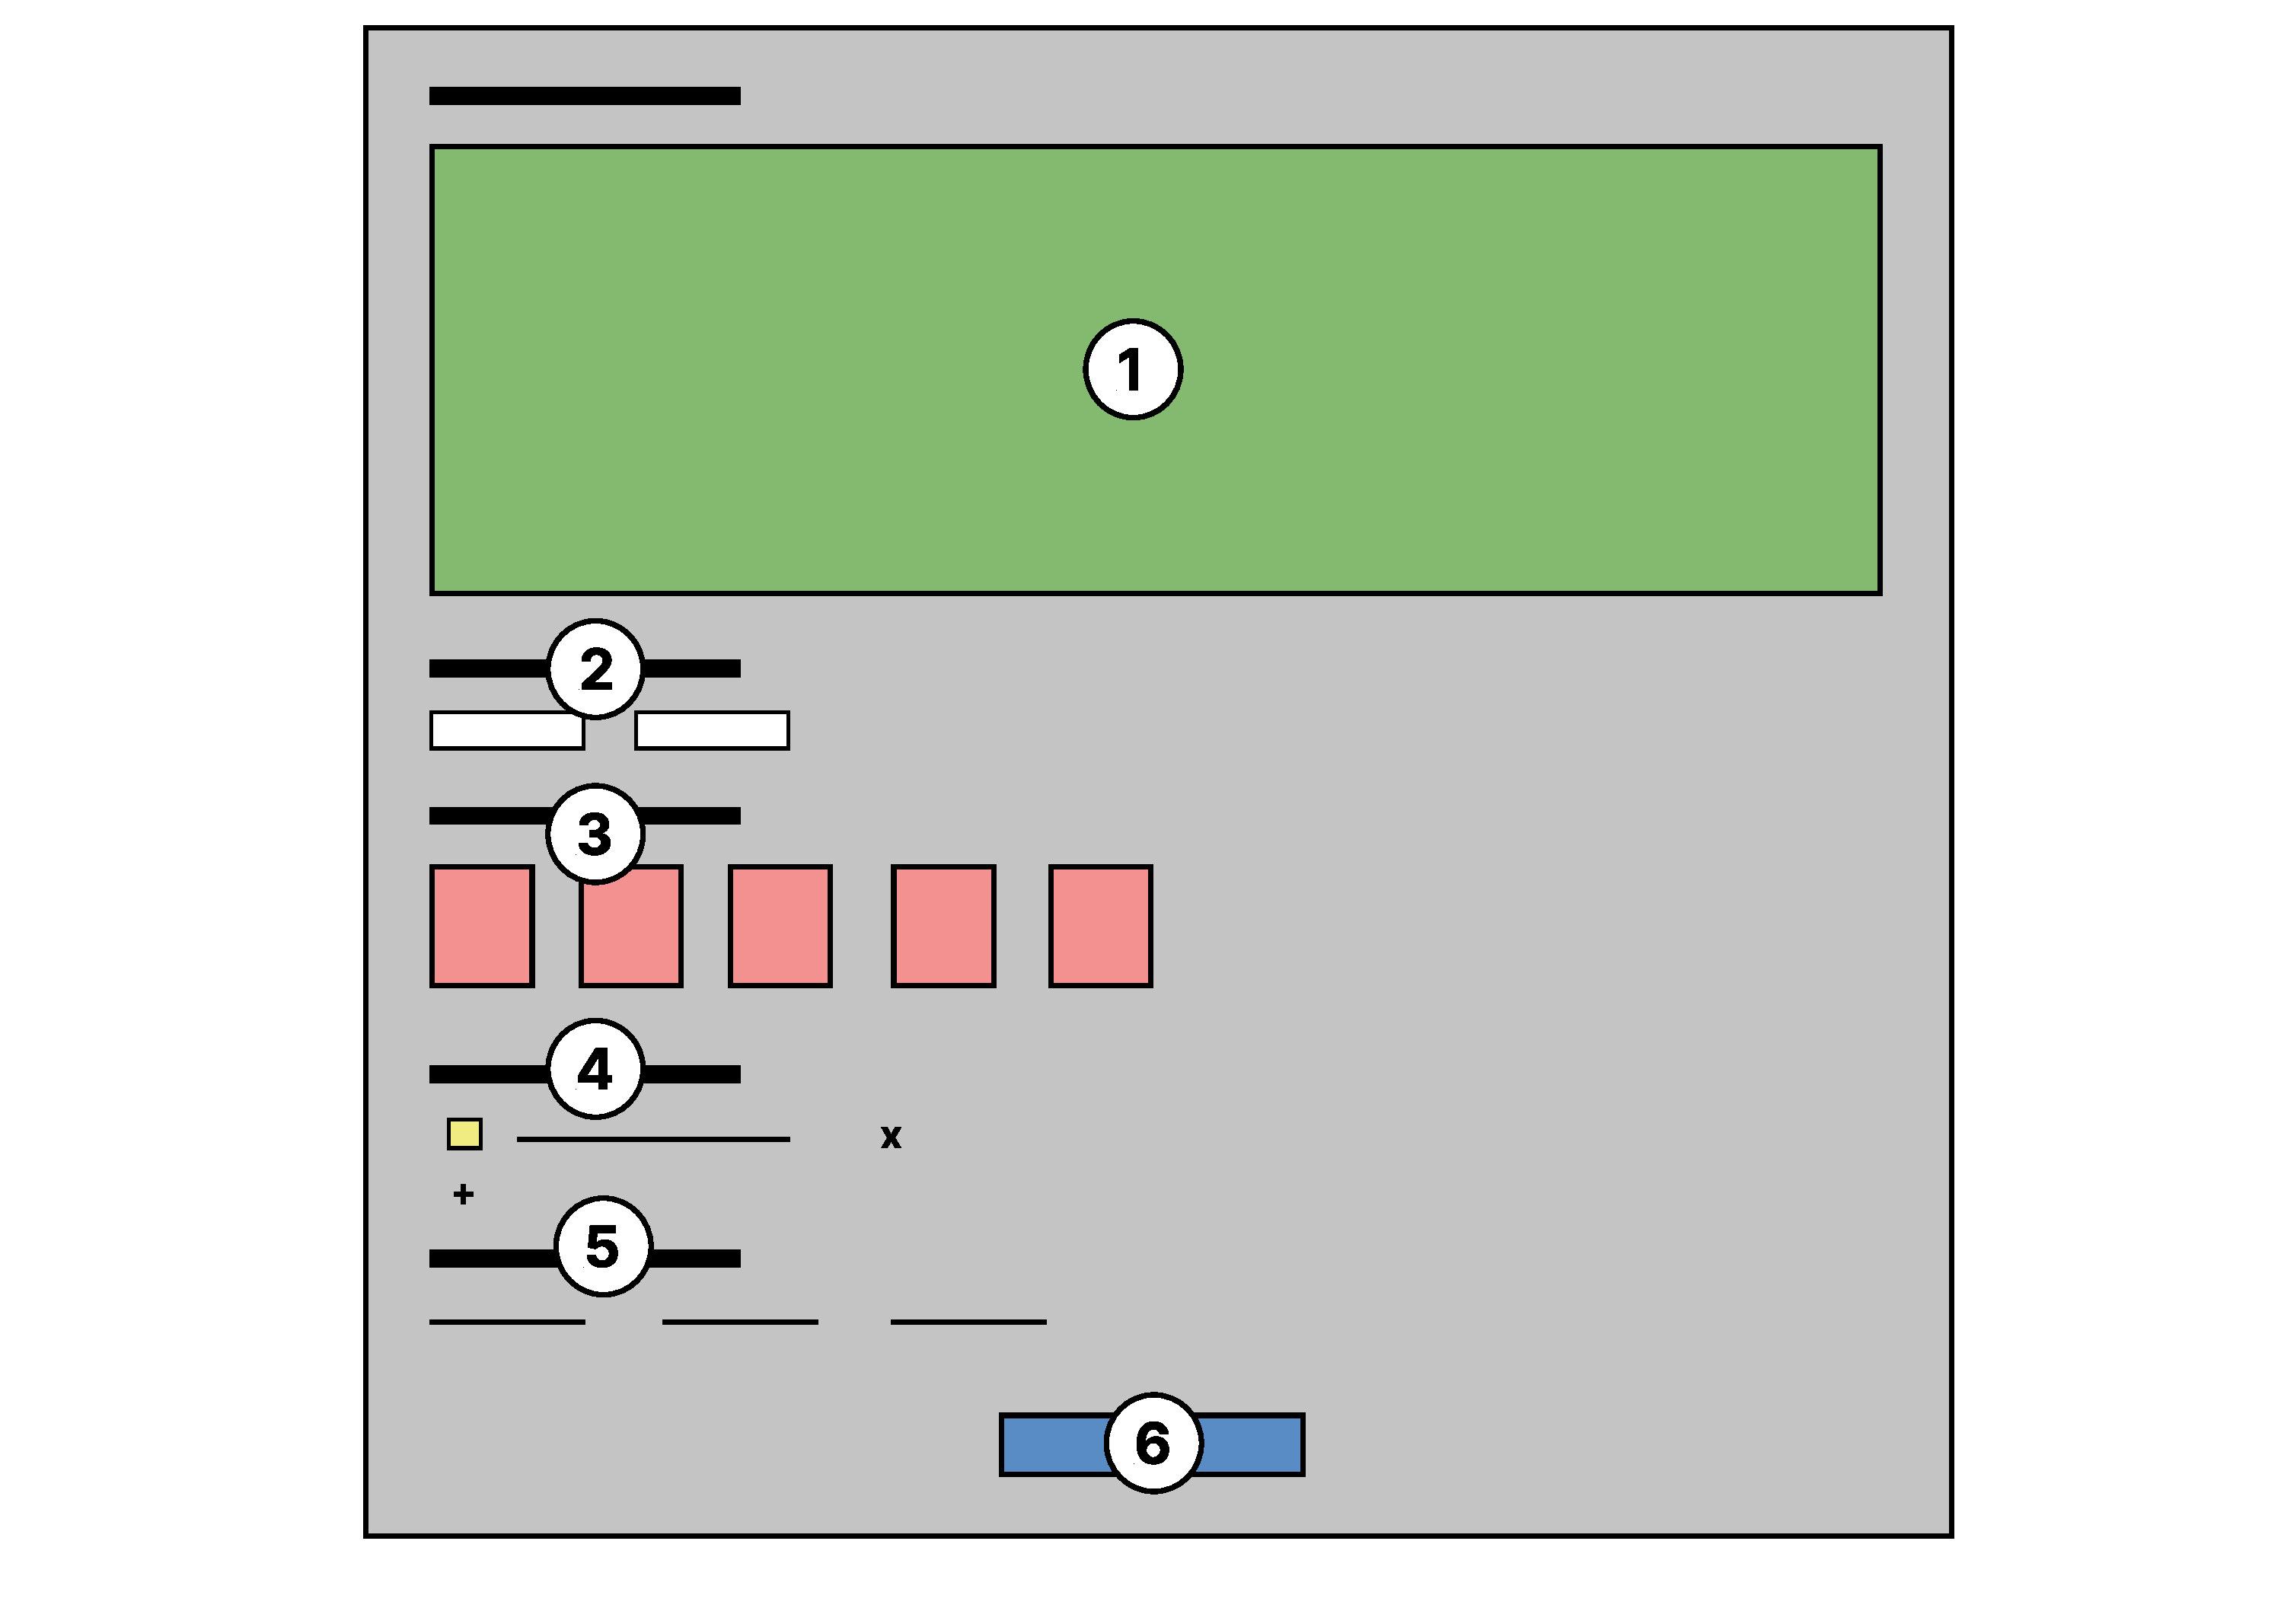
\includegraphics[width=0.6\textwidth]{obrazky-figures/prototype_map.pdf}
	\caption{Návrh užívateľského rozhrania pre tvorbu viac-menej slepej mapy. Najdôležitejším parametrom je voľba územia, označená č. 1, ktorej realizácia bola navrhnutá pomocou ohraničenia žiadaného územia na vloženej mape. Nasleduje nastavenie fyzického rozmeru (č. 2), voľba typu mapy (č. 3), priestor pre vloženie GPX trás (č. 4) a~voľba výstupného formátu (č. 5). Tento návrh bol neskôr ešte rozšírený o~niekoľko ďalších nastavení mapy. Číslom 6 je označené tlačidlo na potvrdenie nastavení.}
	\label{mockup_map}
\end{figure}

Na základe testovania, ktoré je popísane v~kapitole~\ref{testing_1}, bola tvorba úplnej slepej mapy oddelená od tvorby viac-menej slepých máp. Na obrázku~\ref{mockup_blind} je ilustrovaný návrh tejto časti užívateľského rozhrania. Účelom tohto oddelenia bolo odstránenie nastavení, ktoré nie sú pri tvorbe úplne slepých mapách potrebné a~tiež zmena princípu voľby územia.

\begin{figure}[hbt]
	\centering
	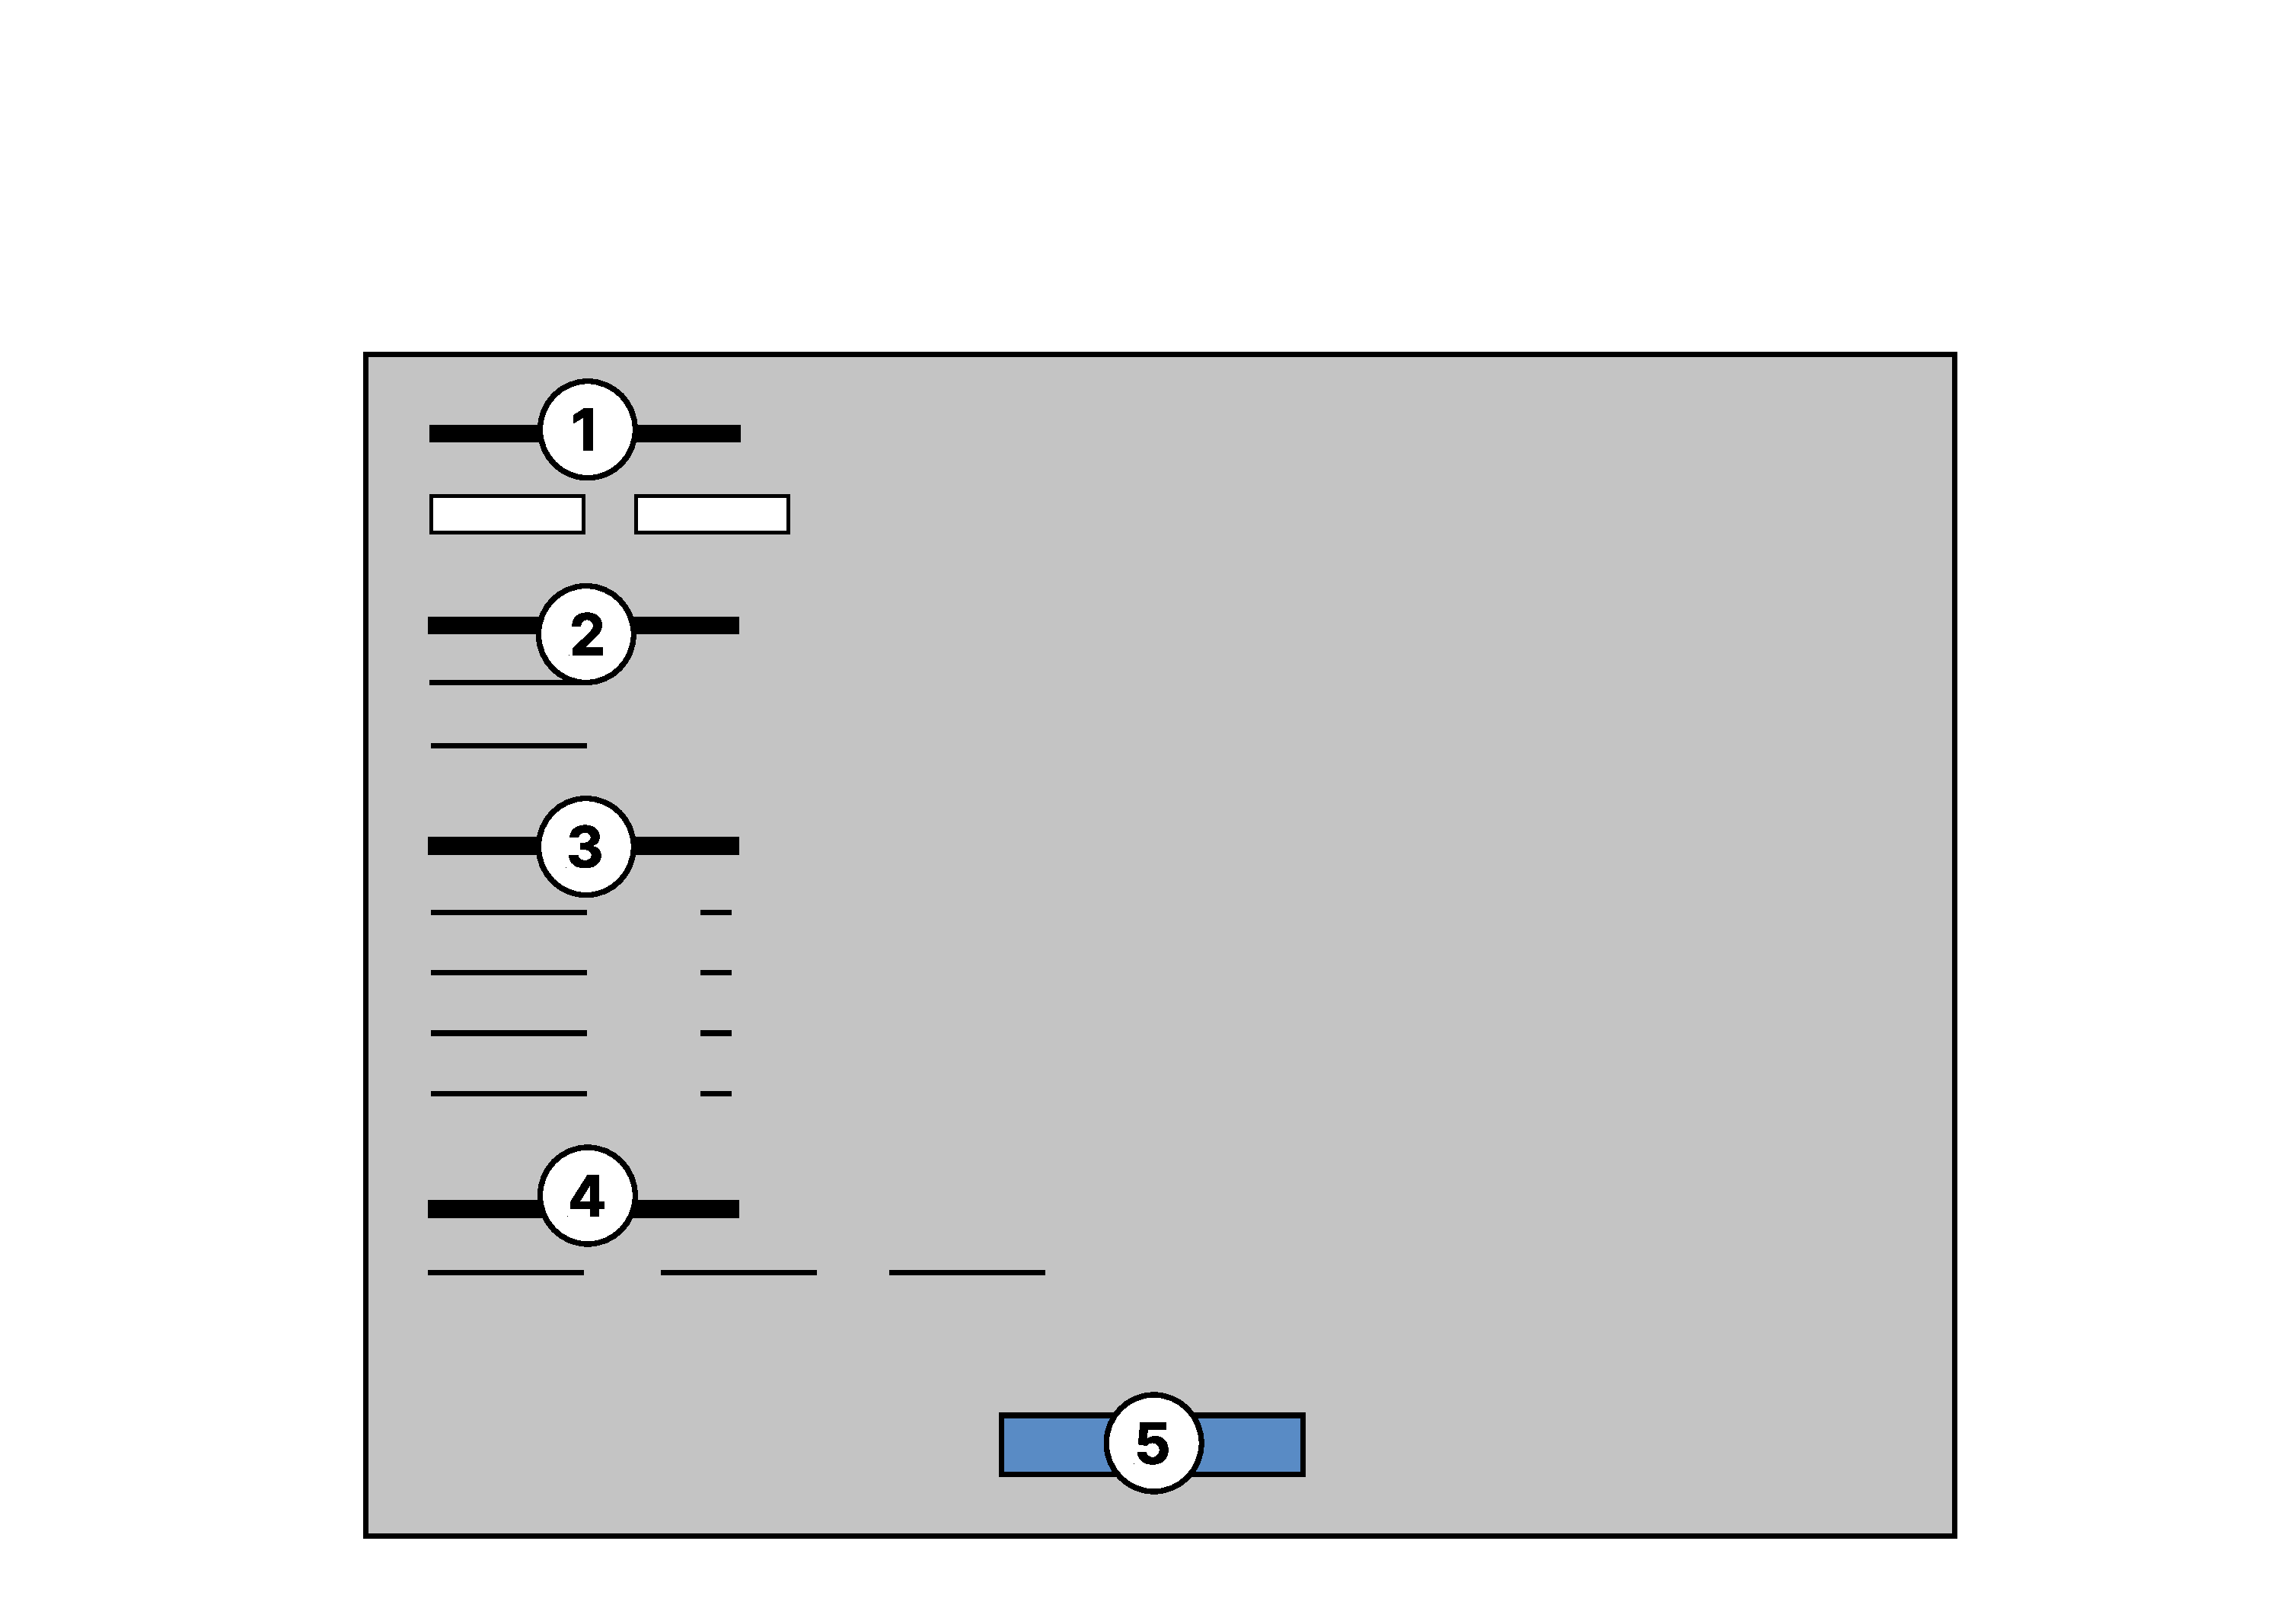
\includegraphics[width=0.6\textwidth]{obrazky-figures/prototype_blind.pdf}
	\caption{Návrh užívateľského rozhrania pre tvorbu úplne slepej mapy. Voľba územia (č.2) je realizovaná v~podobe voľby územného celku -- štátu. Voľba vykreslených prvkov je označená ako č. 3.}
	\label{mockup_blind}
\end{figure}


\subsection*{Tvorba štýlovej sady}
Vytvorený bol aj návrh užívateľského rozhrania pre tvorbu štýlovej sady zobrazený na ľavom obrázku~\ref{mockup_style}. Tvorba štýlovej sady sa skladá z~voľby žiadaných prvkov a~prípadného nastavenia ich detailu. Jednotlivé prvky je možné na základe ich typu rozdeliť do skupín. Tieto tematické skupiny sú v~návrhu reprezentované sekciami, ktoré je možné zbaliť a~rozbaliť. V~sekciách sa nachádzajú nastavenia pre jednotlivé prvky. Nastavenie prvku spočíva v~zvolení úrovne detailu vykreslenia, pričom pod touto voľbou sa nachádza text, ktorý vysvetľuje zvolenú úroveň. Tento text síce popisuje, čo daná úroveň znamená, mapa je ale vizuálne dielo a~preto používateľ pri jej vytváraní potrebuje aj vizuálny vnem, na základe ktorého vie ako bude mapa v~skutočnosti vyzerať. Túto úlohu spĺňa náhľad, ktorý bol v~prvej verzii návrhu umiestnený ako \uv{prilepený} prvok, ktorý pri pohybe na stránke nemenil miesto v~rámci viditeľnej časti stránky.

\begin{figure}[hbt]
	\centering
	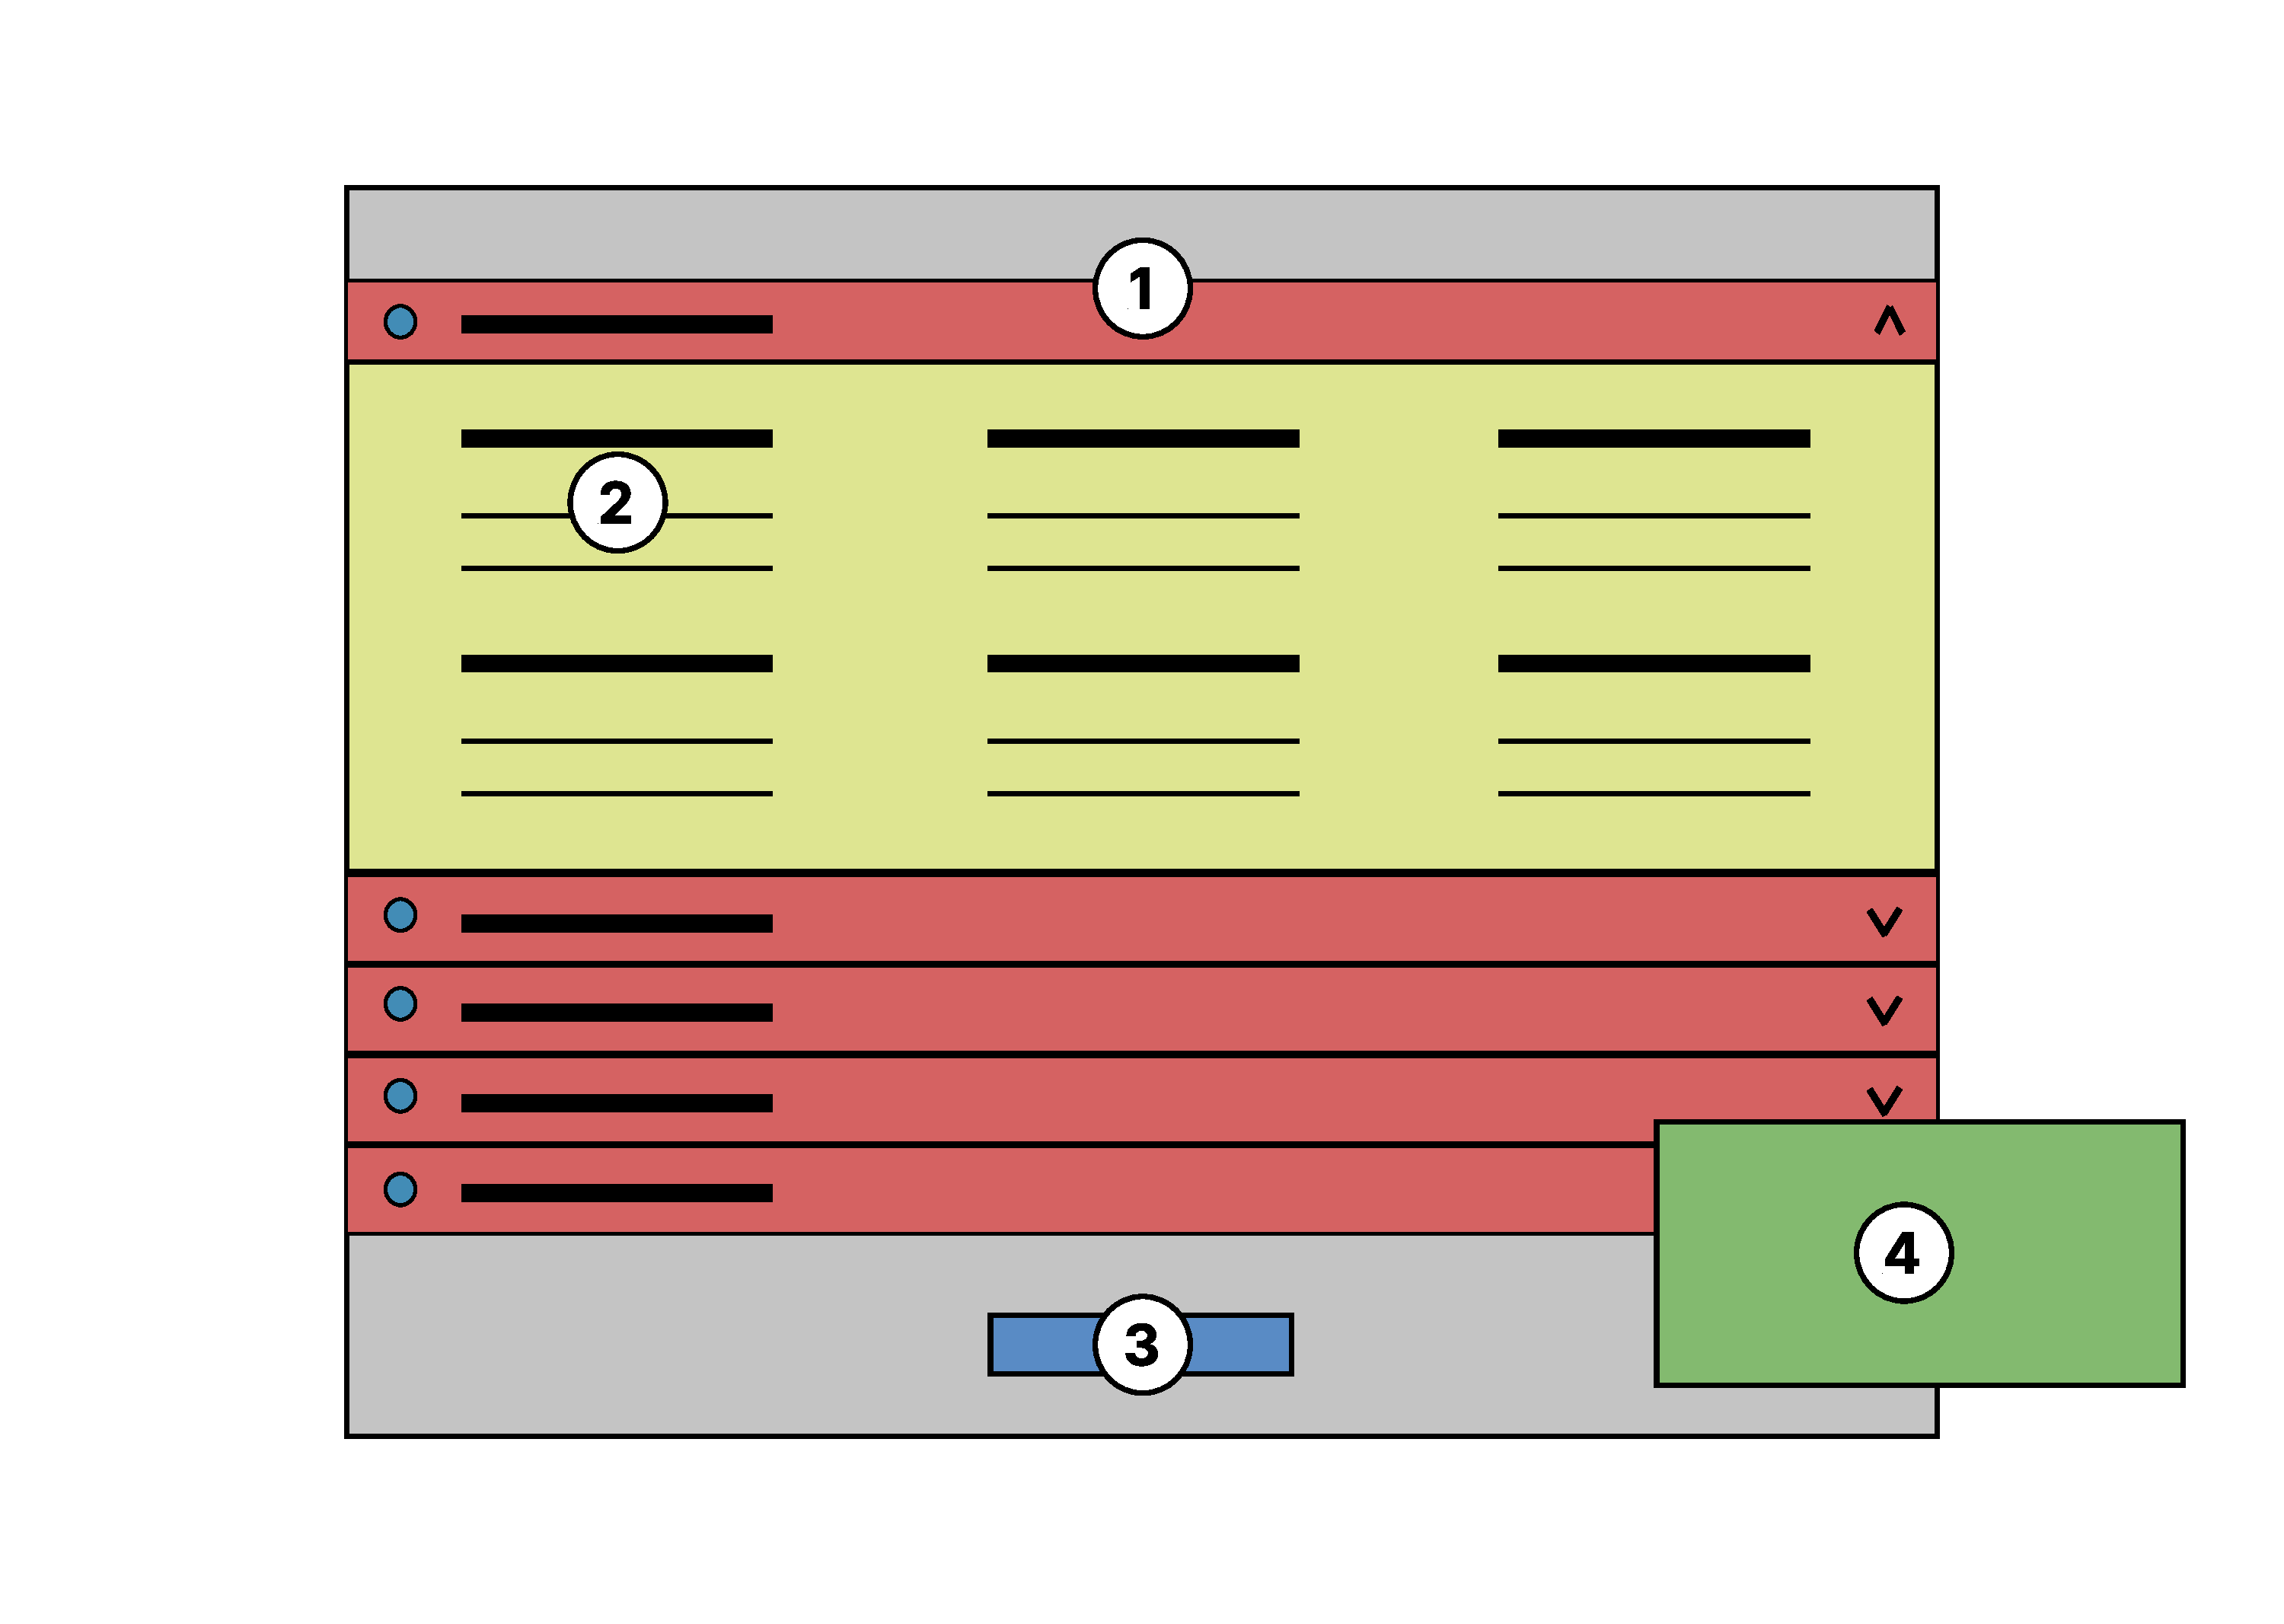
\includegraphics[width=0.5\textwidth]{obrazky-figures/prototype_style_1.pdf}\hfill
	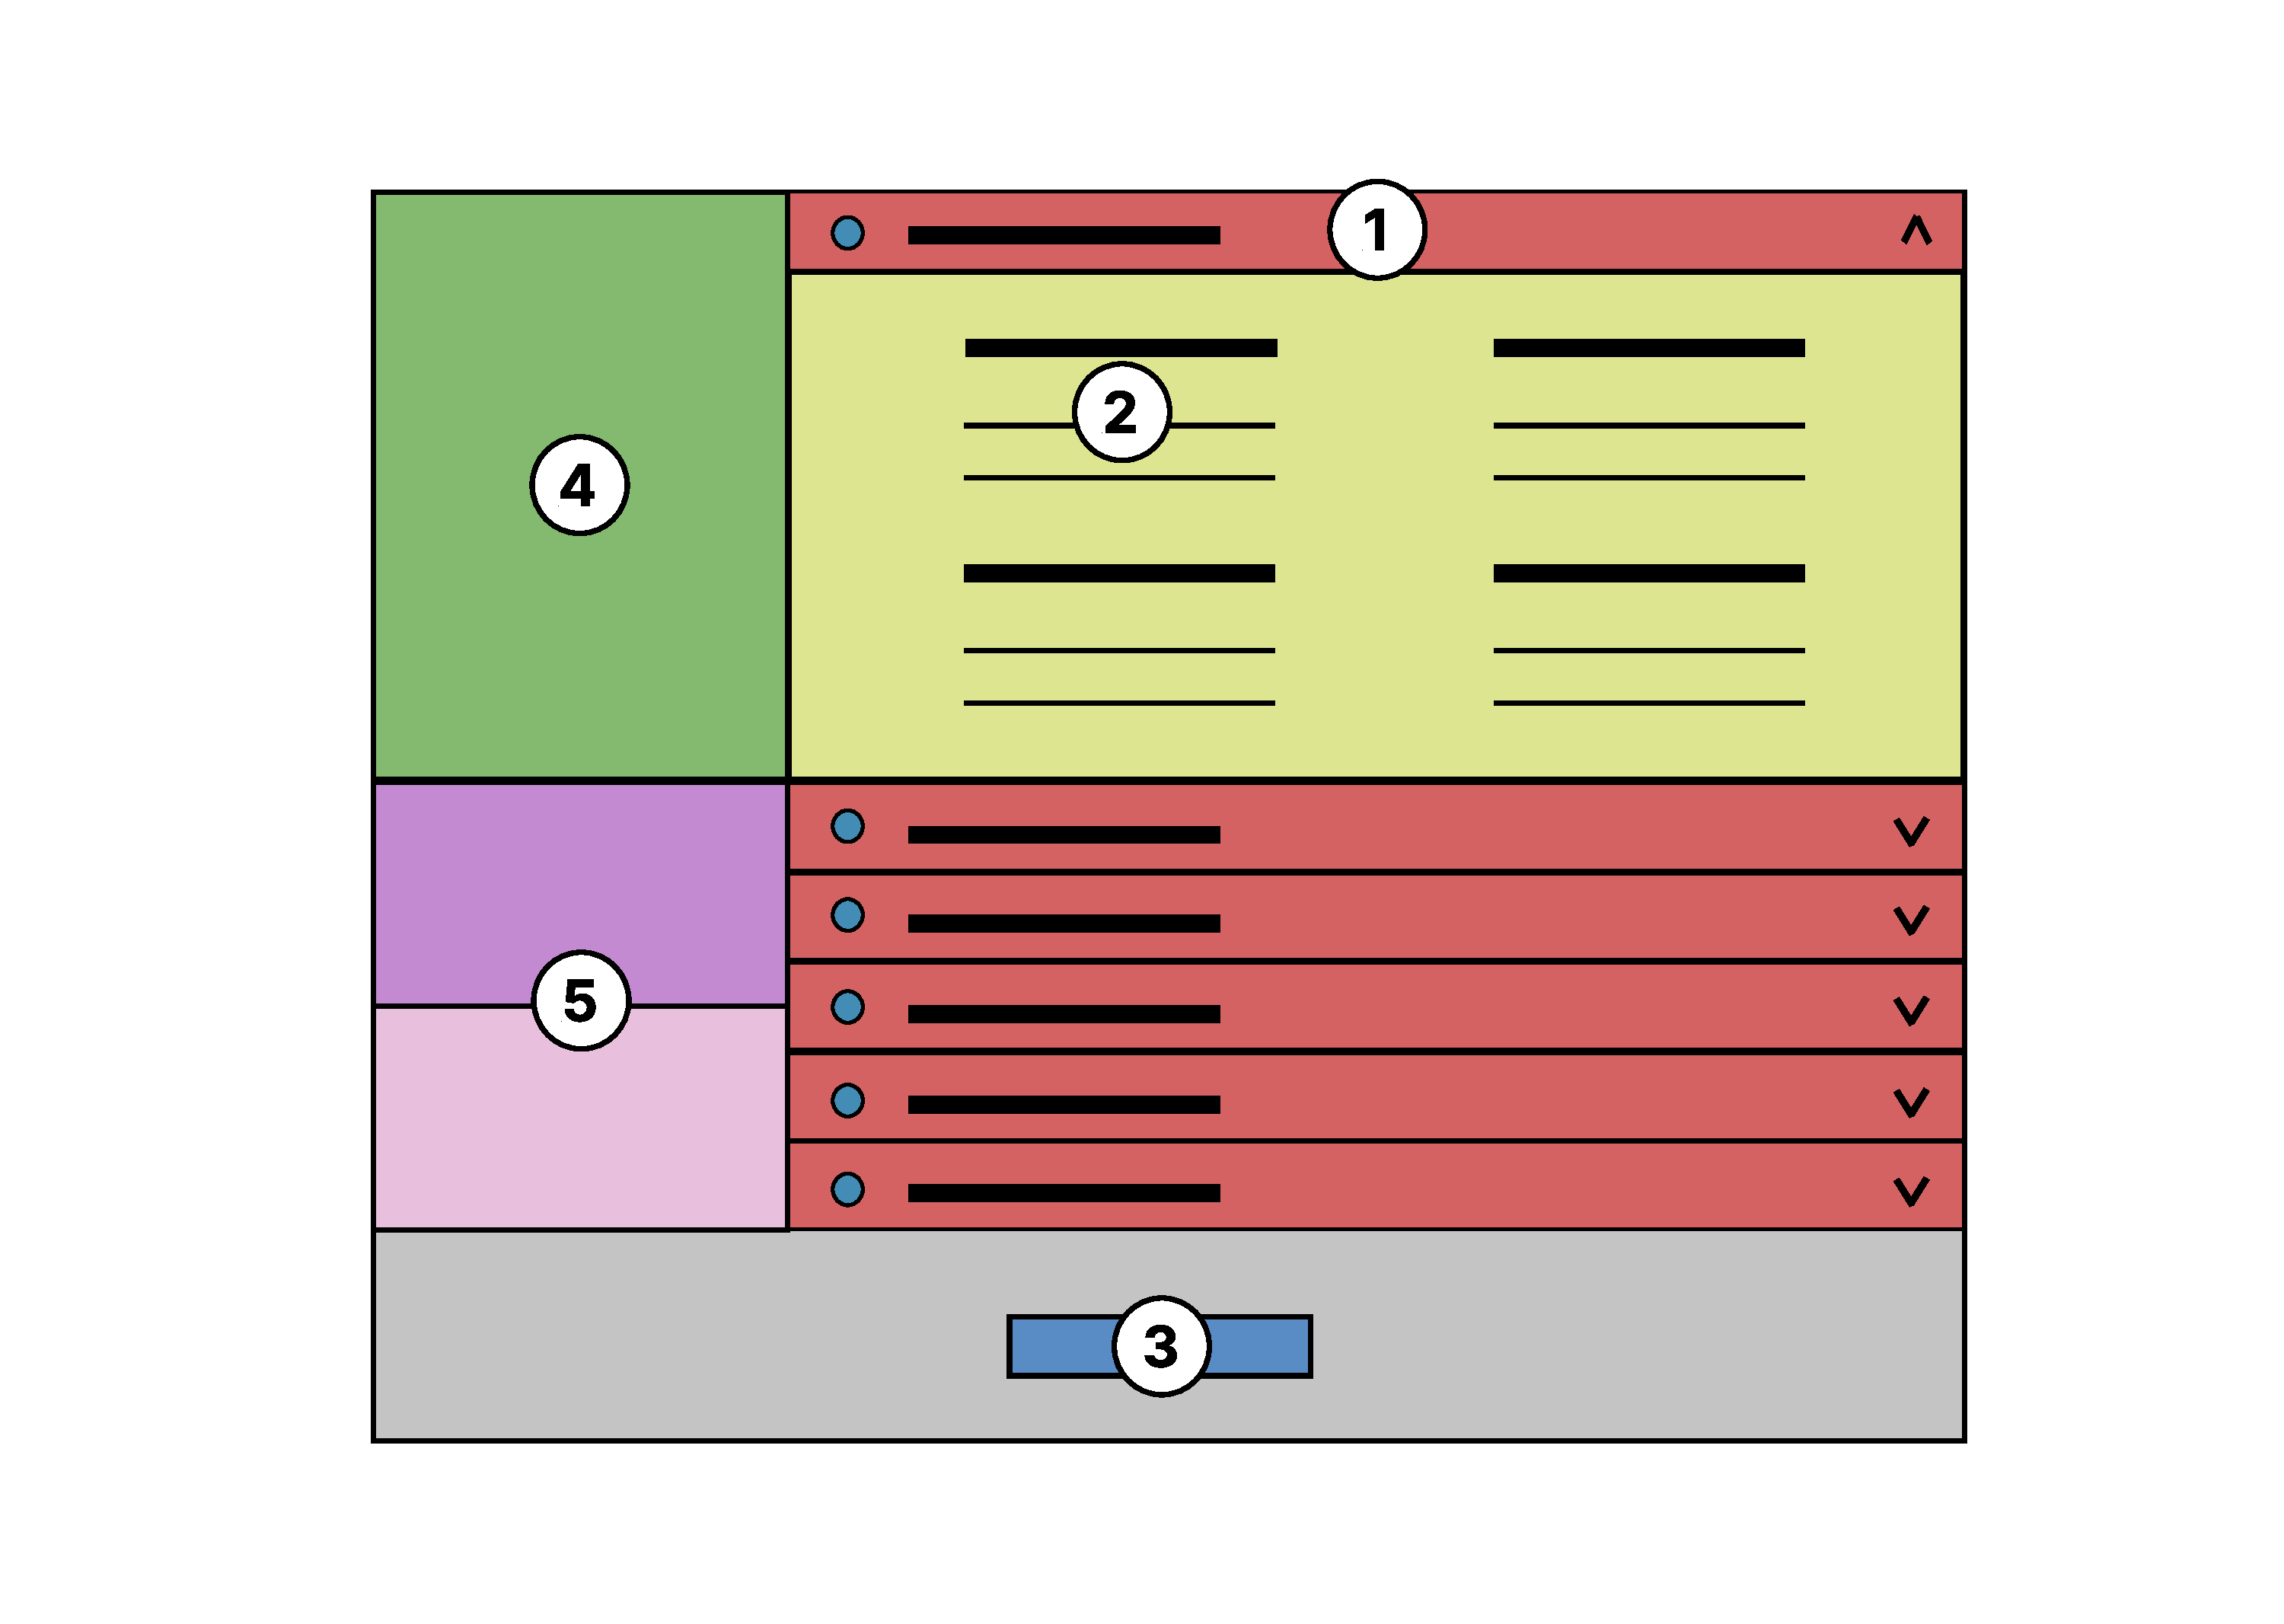
\includegraphics[width=0.5\textwidth]{obrazky-figures/prototype_style_2.pdf}\hfill
	\caption{Prvá a~druhá iterácia návrhu užívateľského rozhrania pre tvorbu štýlovej sady. Iterácie sa líšia hlavne polohou náhľadu.}
	\label{mockup_style}
\end{figure}

Pri testovaní aplikácie však bolo zistené, že pozícia náhľadu nie je vhodná. Z~toho dôvodu bol vytvorený nový návrh užívateľského rozhrania pre tvorbu štýlovej sady, ktorý je zobrazený na pravom obrázku~\ref{mockup_style}. Pri tvorbe tohto návrhu bolo zohľadnené, že náhľad ako reprezentácia mapy, ktorá je vizuálnym médiom by mal mať v~rámci užívateľského rozhrania viac centrálnu úlohu. Preto bolo užívateľské rozhranie rozdelené na dva pomyselné panely, kde na menšom ľavom paneli bol umiestnený spomínaný náhľad a~rozmernejší pravý panel tvorí samostatný výber prvkov. Z~dôvodu veľkého počtu prvkov dostupných vo výbere, spôsobujúceho väčšiu dĺžku tohto panelu, bol tento navrhnutý ako scrollovateľný. Na ľavý panel boli ešte umiestnené ďalšie doplnkové možnosti ako možnosť importu už existujúcej štýlovej sady.


\chapter{Implementácia aplikácie}
\label{implementation}

\section{Získanie dát}
Aplikácia používa dáta z~projektu OpenStreetMap. V~prvej verzií aplikácia získavala dáta pomocou posielania dotazov na Overpass API pomocou knižnice jazyku Python, Python Overpass API. Táto metóda však bola nespoľahlivá a~vyžadovala ďalšiu manipuláciu s~dátami. Pri vývoji aplikácie bolo teda prejdené na prístup uloženia dát do databáze. 

Na stiahnutie dát bol využitý server Geofabrik.de, ktorý ponúka extrakt dát konkrétnych území z~projektu OpenStreetMap. Keďže sa aplikácia zameriava na územie Slovenska a~Českej republiky, bol bol pre každú z~týchto krajín stiahnutý súbor typu {\it .osm.pbf}.

Na vytvorenie jedného súboru, ktorý by obsahoval dáta pre obidve krajiny a~mohol by byť importovaný do databázy bol využitý nástroj osmium a~jeho príkaz {\tt merge}.

Na import do databázy bol využitý nástroj osm2pgsql s~nastavením zachovania multigeometrických prvkov. Dáta boli uložené v~súradnicovom systéme WGS84\footnote{\bf WGS 84 \rm -- Svetový geodetický systém 1984 je štandartom GPS a je založený na geografickej šírke a~dĺžke.}. Pomocou súboru  {\it default.style} bolo nastavené vkladanie prvkov s~niektorými atribútmi do tabuľky pre mnohouholníky namiesto tabuľky pre línie a~tiež pridané stĺpce pre špeciálne atribúty používané pri popise bežne nezobrazovaných prvkov ako turistické alebo lyžiarske trasy.

\section{Uloženie dát}
Na uloženie dát bol využitý databázový systém PostgreSQL s~geo-priestorovým rozšírením PostGIS. Pomocou nástroju osm2pgsql boli prvky na základe ich typu uložené do troch tabuliek: {\it planet\_osm\_point}, {\it planet\_osm\_line}, {\it planet\_osm\_polygon}. Tieto tabuľky sú využívané ako zdroj dát pri tvorbe viac-menej slepej mapy.

\subsection*{Databázové indexy}
\label{indexes}
Za účelom zrýchlenia databázových dotazov bolo vytvorených niekoľko databázových indexov. Indexy boli
vytvorené s~využitím číselnej reprezentácie hodnôt stĺpcov, ktoré sú využívané na zoradenie prvkov ako stĺpec obsahujúci nadmorskú výšku alebo stĺpec obsahujúci údaj o~počte obyvateľov. Indexy boli tiež vytvorené s~využitím kombinácie stĺpca identifikujúceho druh cesty, resp. stĺpca identifikujúceho druh železnice a~stĺpca určujúceho úroveň. Táto kombinácia je totiž využívaná veľmi často pri vykresľovaní všetkých úrovní mostov rôznych typov ciest, resp. železníc. Taktiež bol vytvorený index s~využitím výpočtu územia prvku pomocou funkcie {\tt ST\_Area}, ktorý je využívaný pri selekcií území dostatočne veľkých na vykreslenie.

\subsection*{Úplne slepá mapa}
Pri úplnej slepej mape je cieľom zobraziť len prvky konkrétneho územia -- štátu. Je preto potrebné so zvolenej množiny prvkov odstrániť tie, ktoré sa nachádzajú mimo toto územie. Pri prvkoch typu línia, ako napríklad rieky, je tiež žiadúce tieto prvky zobraziť len v~rámci zvoleného územia, a~teda je potrebné ich orezať. 

Toto je možné realizovať pomocou mnohých dostupných funkcií rozšírenia PostGIS. Keďže však úplne slepé mapy môžu obsahovať len neveľkú a~nemennú množinu prvkov, nedáva zmysel zakaždým vykonávať tie isté operácie, ktoré navyše výrazne spomaľujú proces tvorby mapy. Z~toho dôvodu boli vytvorené samostatné tabuľky {\it blind\_point}, {\it blind\_line} a~{\it blind\_polygon}, ktoré obsahujú len prvky používané pri tvorbe úplne slepých máp. Pri importe do nových tabuliek boli navyše vynechané prvky, ktoré sa nachádzajú mimo zobrazovaných území a~prvky presahujúce vykresľované územia boli orezané. V~nových tabuľkách bol tiež pre zrýchlenie výberu prvkov pre každé zobrazované územie pridaný stĺpec obsahujúci pravdivostné hodnoty popisujúce príslušnosť prvku do daného územia. Porovnanie získania dát z~rôznych databázových tabuliek a~s použitím rôznych funkcií je zobrazené v~tabuľke~\ref{db_compare}.

Na výber len prvkov nachádzajúcich sa vo voliteľných územiach boli využité funkcie rozšírenia PostGIS, kde jeden argument tvoril daný prvok a~druhý konkrétne územie. Pomocou funkcie {\tt ST\_Within()} boli vybraté prvky nachádzajúce sa celkom vo vnútri územia. Na zvolenie prvkov, ktoré sa nachádzajú blízko pri hraniciach a~miestami ich môžu jemne presahovať bolo v~kombinácií s~touto funkciou použité porovnanie veľkostí územia prieniku a~územia rozdielu pomocou funkcií {\tt ST\_Intersection()}, {\tt ST\_Difference()} a~{\tt ST\_Area()}. Na orezanie presahujúcich prvkov typu línia bola použitá funkcia {\tt ST\_Intersection()} v~kombinácií s~funkciou {\tt ST\_Crosses()} pomocou, ktorej boli získané prvky prekračujúce hranice územia.

\begin{table}[hbt]
	\centering
    \begin{tabular}{|l|c|c|c|}
        \hline
        \bf Databázová tabuľka & \bf Použité funkcie & \bf Počet prvkov & \bf Čas vykonania \rm \\
        \hline
        planet\_osm\_polygon & žiadne & 61 & 4.477 ms \\
        \hline
        planet\_osm\_polygon & ST\_Intersects() & 28 & 2 770.245 ms \\
        \hline
        planet\_osm\_polygon & ST\_Within() & 11 & 2 648.407 ms \\
        \hline
        planet\_osm\_polygon & ST\_Within() & 13 & 14 317.965 ms \\
        & + ST\_Intersection() & & \\
        & a~ST\_Difference() & & \\
        \hline
        blind\_polygon & žiadne & 13 & 0.293 ms \\
        \hline
    \end{tabular}
    \vskip6pt
	\caption{Porovnanie rôznych spôsobov získavania dát pre úplne slepé mapy. Porovnaný je priemerný čas vykonania a~počet získaných prvkov pre dotazy na prvky popisujúce národné parky na území Slovenska a~Českej republiky. Dotazy s~využitím funkcií nie sú optimalizované, takže ich čas má potenciál byť čiastočne nižší. Na Slovensku sa nachádza 9 národných parkov a~na území Českej republiky sú 4, čo činí 13 národných parkov na spoločnom územií. V~počte prvkov sú národné parky tvorené viacerými prvkami zahrnuté len jeden krát.}
    \vskip6pt
	\label{db_compare}
\end{table}

\section{Proces tvorby mapy}
Generovanie mapy je podobne ako užívateľské rozhranie rozdelené na tvorbu viac-menej slepých máp a~tvorbu úplne slepých máp. Princíp je u~obidvoch podobný, no líšia sa nastaveniami mapy a~tiež používajú rôzne vrstvy, zdroje dát a~štýly. Tvorba úplne slepej mapy je priblížená v~kapitole~\ref{implementation_blind}. Prvky mapy sú definované programovo, s~výnimkou definícií štýlov, ktoré sú vytvorené pomocou súborov typu XML. Mapa je vygenerovaná do súboru, ktorého obsah je načítaný a zakódovaný do formátu base64. Načítané dáta sú v~odpovedi odoslané klientovi, kde sú využité buď na vytvorenie súboru pre stiahnutie alebo zobrazenie mapy, ak sa jedná o~náhľad.

Implementácia tvorby viac-menej slepej mapy sa nachádza v~súbore {\tt map.py}. Ústredným bodom je funkcia {\tt make\_map()}, ktorá je volaná pri zaznamenaní požiadavku na tvorbu mapy.

\subsection*{Základné parametre mapy}
Proces tvorby mapy začína vytvorením objektu triedy {\tt Map} s~definovaním fyzického rozmeru mapy a~použitej projekcie. Ďalej je potrebné definovať územie zobrazené na mape. O~toto sa stará vlastná funkcia {\tt get\_bbox()}, ktorá transformuje zvolené hraničné súradnice mapy v~systéme WGS84 do súradníc systému použitej projekcie a~vráti objekt triedy {\tt Box2d} reprezentujúci obálku mapy. Pomocou funkcie knižnice Mapnik {\tt zoom\_to\_bbox()} je následne mapa upriamená na toto územie.

Po nastavení geografického a~fyzického rozmeru mapy, je už zrejmá jej mierka, ktorú je možné získať pomocou funkcie {\tt Map.scale()}. Na základe mierky je následne určené, do ktorej úrovne priblíženia mapa spadá. Program interne používa deväť úrovní priblíženia, ktoré pokrývajú celé dostupné spektrum hodnôt mierky. Na základe úrovne priblíženia je určená hodnota faktoru priblíženia, ktorá je uložená do premennej {\tt zoom\_factor}. Význam tejto hodnoty je bližšie objasnený v~kapitole~\ref{styles}. Úroveň priblíženia je tiež používaná pri výbere prvkov a~ich spôsobe vykreslenia.

\subsection*{Štýlová sada}
Tvorba mapy pokračuje nastavením štýlovej sady. V~prípade použitia jednej zo šablón je definícia tejto šablóny načítaná z~príslušného súboru typu JSON. Jednotlivé nastavenia sú ešte pred použitím prispôsobené úrovni priblíženia mapy. Prispôsobenie úrovni priblíženia je bližšie popísané v~kapitole~\ref{adjust_to_zoom}. V~prípade použitia vlastnej štýlovej sady, musí byť jej definícia súčasťou požiadavku na vytvorenie mapy.

Program pokračuje načítaním súboru typu XML obsahujúceho definície štýlových pravidiel. Obsah tohto súboru je najprv načítaný do reťazca a~na základe nastavení mapy je ešte prípadne prispôsobený. Prispôsobenie štýlových pravidiel sa týka najmä úpravy farieb povrchu mapy na základe farebnej témy zvolenej štýlovej sady a~nastavenia hraničných hodnôt veľkostí území na základe úrovne priblíženia. Hraničné hodnoty veľkostí území prvkov sú použité na filtrovanie prvkov pri voľbe veľkosti a~umiestnenia popisu týchto prvkov. Tieto štýlové pravidlá sú potom pridané do mapy pomocou funkcie {\tt Map.load\_map\_from\_string()}.

\subsection*{Výber vrstiev a~štýlov}
Aby mapa mala vôbec čo zobrazovať, je potrebné pridať do nej vrstvy. Vrstvy sú uložené v~dátovej štruktúre jazyka Python typu slovník (angl. dictionary). V~tomto slovníku sú definované všetky vrstvy definujúce vykreslenie všetkých aplikáciou podporovaných prvkov mapy. Pre každú vrstvu je definované jej poradové číslo určujúce poradie pri vykresľovaní, pole so štýlmi dostupnými pre túto vrstvu a~databázový dotaz na získanie dát danej vrstvy z~databázy s~rozšírením PostGIS.

Databázové dotazy niektorých vrstiev závisia od nastavení iných prvkov, a~preto obsahujú zástupný formátovací symbol, ktorý musí byť pri zvolení vrstvy nahradený. Tieto vrstvy potom v~slovníku obsahujú aj ďalšiu hodnotu, ktorá značí čím má byť zástupný symbol nahradený. Takýmto spôsobom fungujú napríklad vrstvy vykresľujúce bežne cesty, ktoré na základe vypnutia alebo zapnutia voľby vykreslenia tunelov alebo mostov, zahŕňajú alebo nezahŕňajú aj cesty v~tuneloch alebo na mostoch.

Jednotlivé vrstvy sú vyberané na základe ďalšieho slovníka, v~ktorom je pre každú úroveň detailu každého dostupného nastavenia v~nástroji tvorby štýlovej sady, uložený slovník obsahujúci zoznam vrstiev, ktoré táto úroveň detailu aktivuje a~štýlov, ktoré majú byť na prvky týchto vrstiev aplikované. Zvolené vrstvy sú ukladané do poľa, ktoré je po pridaní poslednej vrstvy zoradené na základe poradových čísiel vrstiev. 

Pre zvolené vrstvy sú následne postupne programovo vytvorené objekty triedy {\tt Layer}, ktoré sú postupne pridávané do mapy. Pre zdroj dát každej vrstvy je okrem parametrov pripojenia k~databáze určená aj obálka limitujúca výber prvkov iba na žiadané územie a~výrazne tak znižujúca čas generovania mapy. Pri Mercatorovom zobrazení je použitá obálka mapy a pri Křovákovom zobrazení je použitá rozšírená obálka mapy, ktorá je bližšie vysvetlená v~ďalšej kapitole~\ref{krovak_pad}.

\subsection*{Křovákove zobrazenie}
\label{krovak_pad}
Keďže Křovákove zobrazenie je voči Mercatorovmu zobrazeniu pootočené, mapa v~tomto zobrazení je tiež pootočená. Pri vygenerovaní takejto mapy preto vzniknú v~jej rohoch trojuholníkové územia, ktoré nie sú vykreslené, čo je možné pozorovať na obrázku~\ref{img_krovak_pad}. Tento problém by sa dal vyriešiť orezaním mapy, tak aby tieto územia neboli zobrazené. To by však znamenalo, že mapa zobrazuje menšie územie ako má. Preto je najlepším riešením rozšíriť územie, ktorého prvky sú vykreslené tak, aby bola vykreslená celá výsledná mapa. Potrebné hodnoty rozšírenia územia do jednotlivých smerov je možné na základe uhlu pootočenia vypočítať pomocou jednoduchých geometrických výpočtov.

\begin{figure}[hbt]
	\centering
	\includegraphics[width=0.8\textwidth]{obrazky-figures/krovak_bad.pdf}
	\caption{Mapa s~použitím Křovákovho zobrazenia bez rozšírenia obálky ohraničujúcej územie, z~ktorého sú vyberané prvky mapy. Čierny obdĺžnik vykresľuje obálku mapy v~súradniciach Křovákovho zobrazenia. Mapa je vygenerovaná pomocou vytvorenej aplikácie.}
	\label{img_krovak_pad}
\end{figure}

\subsection*{Vykreslenie importovaných trás}
V prípade, že požiadavok o~vykreslenie mapy obsahuje priložené trasy v~súboroch typu GPX, program musí vytvoriť vrstvy aj pre tieto trasy. Keďže pre vložené trasy je možné zvoliť aj ľubovoľnú farbu, pre tieto trasy je nutné programovo definovať aj štýl vykreslenia. 

Pre všetky súbory typu GPX sú postupne vytvorené štýly a~vrstvy, ktoré sú v~správnom poradí vložené do mapy. Na načítanie trás vo formáte GPX je použitý zásuvný modul Ogr a~voľba vrstvy {\it tracks}, ktorá označuje trasy. 

\subsection*{Vygenerovanie výstupu}
Keď sú do mapy pridané všetky vrstvy, ktoré majú byť vykreslené, mapa je takmer pripravená na vygenerovanie. Posledným úkonom je vypočítanie hodnoty tzv. faktoru mierky (angl. scale factor). Táto premenná určuje akou hodnotou budú prenásobené veľkosti vykreslenia prvkov. Vypočíta sa ako podiel nastavenej hodnoty DPI a~implicitnej hodnoty DPI použitej v~knižnici Mapnik -- 90.7. Pri nastavení 300 DPI miesto 90.7 pri rovnakom rozmere tak budú objekty vykreslené približne tri krát väčšie, čo dorovnáva skutočnosť, že na papieri bude takáto mapa vykreslená približne tri krát menšia. Faktor mierky je ešte prenásobený faktorom priblíženia, ktorý je bližšie objasnený v~kapitole~\ref{styles}.

Keďže Mapnik umožňuje generovanie mapy len do súboru, je potrebné predísť prepisu ďaľších súborov. Na vygenerovanie mena výstupného súboru je preto použitá metóda {\tt uuid4()} z~knižnice UUID a~jej výstup je prevedený na hexadecimálny reťazec. Táto funkcia generuje všeobecne unikátne identifikátory, ktoré síce nezaručujú unikátnosť no pravdepodobnosť výskytu kolízie v~103 biliónoch opakovaní je približne jedna ku miliarde.~\cite{uuid}

Následne je s~aplikovaním faktoru mierky vygenerovaná mapa, ktorá je uložená do súboru. 

\subsection*{Tvorba úplnej slepej mapy}
\label{implementation_blind}
Tvorba úplne slepej mapy je implementovaná v~súbore {\tt blind\_map.py}. Na rozdiel od tvorby viac-menej slepých máp implicitne využíva Mercatorovo zobrazenie. Výstupný formát je zvolený na základe voľby použitia mapy. Pri voľbe digitálneho použitia mapy je zvolený rastrový formát PNG a~pri voľbe použitia na tlač je použitý vektorový formát PDF, vďaka čomu nie je potrebné riešiť nastavenie hodnoty DPI. 

Rozdielna je tiež voľba fyzického a~geografického rozmeru mapy. Fyzický rozmer je určený voľbou jedného zo zaužívaných formátov, ktoré sú v~programe konvertované na pixely. Geografický rozmer je určený voľbou štátov. Program na základe definovaných obálok týchto štátov určí obálku mapy. 

Vrstvy sú definované v~špeciálnom slovníku a~ich definícia sa skladá z~poradového čísla, názvu štýlu, a~databázového dotazu. Databázové dotazy tiež obsahujú zástupný formátovací symbol, ktorý je pri voľbe vrstvy nahradený reťazcom obsahujúcim podmienku na kontrolu príslušnosti prvku k~zvoleným územiam -- štátom.

\subsection*{Tvorba náhľadu}
\label{implementation_preview}
Náhľad je generovaný rovnakým spôsobom ako viac-menej slepé mapy, s~tým rozdielom, že používateľ môže nastaviť len jeden parameter, a~tým je územie. Zvyšné parametre sú nastavené implicitne. Keďže je určený na digitálne použitie a~taktiež z~rýchlostných dôvodov, náhľad je generovaný ako súbor typu PNG.

\section{Definícia štýlov}
\label{styles}
Štýly sú definované v~súboroch typu XML. Sú vytvorené so zameraním na úroveň priblíženia číslo 7, ktorá je využitá pre rozpätie mierky mapy od 1 : 17 000 do 1 : 50 000, čo je rozpätie, v ktorom sa bežne pohybuje mierka väčšiny používaných máp ako napríklad turistické alebo cyklistické mapy. 

Pre každú úroveň priblíženia je definovaný tzv. faktor priblíženia (angl. zoom factor), ktorý vyjadruje pomer veľkosti prvkov danej úrovni voči úrovni číslo 7. Týmto číslom je prenásobený tzv. faktor mierky (angl. scale factor), čo je hodnota, ktorou sú vynásobené veľkostné parametre vykreslenia prvkov. Vďaka tomuto riešeniu nie je nutné definovať štýlové pravidlá pre každú úroveň priblíženia a~následne vykonávať množstvo operácií porovnania pri selekcií štýlových pravidiel, ktoré by spomaľovalo činnosť aplikácie.

Program využíva väčšinu dostupných symbolizérov a~pri každom definuje parametre dôležité pri tvorbe prehľadnej a~funkčnej mapy:
\begin{itemize}
  \item{\bf LineSymbolizer \rm - Je využitý na vykreslenie línií. Využíva primárne definíciu farby, hrúbky, priesvitnosti a~ukončenia línie. Na zvýraznenie jemnej odlišnosti alebo hierarchie prvkov sú tiež využívané prerušované línie. Prvky typu línia sú spravidla vykreslené s~použitím viacerých symbolizérov, kde jeden, ktorý je vykreslený ako prvý je hrubší a~vytvára okraj a~druhý je menej hrubý a~tvorí výplň. Pri vykreslení území tiež bolo použité odsadenie jedného symbolizéru za účelom informovania o~vnútornej strane územia.}
  \item{\bf PolygonSymbolizer \rm - Je využitý na vykreslenie výplne mnohouholníkov. Využíva definíciu farby a~prípadne priesvitnosti.}
  \item{\bf TextSymbolizer \rm - Je využívaný na textový popis prvkov, prevažne línií a~mnohouholníkov. Využíva najmä definíciu typu, fontu a~veľkosti písma, maximálnej širky bez zalomenia, hrúbky a~farby obrysu (angl. halo) a~umiestnenia. Využíva bodové umiestnenie pre označenie bodov, pozdĺžne umiestnenie pre označenie línií a~pre označenie mnohouholníkov používa tzv. vnútorné umiestnenie (angl. interior), ktoré zapríčiní umiestnenie textového popisu do vnútra územia mnohouholníku. Pri pozdĺžnom umiestnení využíva tiež definíciu minimálnej dĺžky prvku, vzdialenosti medzi vykreslenými popismi a~veľkosti odsadenia.}
  \item{\bf ShieldSymbolizer \rm - Je využívaný na vykreslenie samotnej ikony alebo ikony v~kombinácií s~textovým popisom pre prvky všetkých typov. Využíva väčšinu textových parametrov, ktoré využíva TextSymbolizer a~pridáva definície transformácie ikony na zmenu veľkosti.}
  \item{\bf LinePatternSymbolizer \rm - Je využitý na vykreslenie línií pomocou ikony. Príležitostne využíva definíciu transformácie na zmenu veľkosti.}
  \item{\bf PolygonPatternSymbolizer \rm - Je využívaný na vykreslenie výplne mnohouholníkov vzorom pomocou ikony.}
  \item{\bf MarkerSymbolizer \rm - Je využitý na vykreslenie ikony ako smerovej značky -- pozdĺž prvku typu línia.}
\end{itemize}

{\it TextSymbolizer} a~{\it ShieldSymbolizer} tiež využívajú definicíu minimálnej vzdialenosti od kraja mapy a~ostatných prvkov, kedy sú ešte vykreslené. Keďže tieto parametre nie sú dostupné pre {\it PointSymbolizer} bol aj pre vykreslenie samostatných ikon použitý {\it ShieldSymbolizer}. Väčšina ikon použitých v aplikácií pochádza zo štýlovej sady používanej v projekte OSM -- OSM Carto, ktorá je dostupná pod licenciou CC0 Public Domain Dedication\footnote{CC0 Public Domain Dedication -- \url{https://creativecommons.org/publicdomain/zero/1.0/}}. Ikony pre ďalšie prvky, ktoré nie sú vykresľované~v OSM Carto, no boli vyhodnotené ako zaujímavé, boli buď vytvorené alebo získané --~a prípadne upravené --~z úložiska ikon SVG Repo\footnote{\url{https://www.svgrepo.com/}} pod rovnakou licenciou. 

V textových popisoch bol zvolený typ písma \bf Merriweather \rm\footnote{\url{https://fonts.google.com/specimen/Merriweather}} z~knižnice fontov \bf Google Fonts\rm\footnote{\url{https://fonts.google.com/}}, ktorý ponúka vhodnú rovnováhu medzi čitateľnosťou a výraznosťou. Tento typ písma je šírený pod licenciou SIL Open Font License\footnote{SIL Open Font License -- \url{https://scripts.sil.org/cms/scripts/page.php?site_id=nrsi&id=OFL}}.

Symbolizéry vykresľujúce línie a~mnohouholníky tiež využívajú definíciu parametru {\tt clip}, v~prípade použitia ktorého, je vytvorený štvoruholníkový prvok popisujúci obálku mapy, na základe ktorého sú orezané geometrie týchto prvkov. Vďaka tomuto nastaveniu nie sú zbytočne vykresľované časti prvkov, ktoré nie sú viditeľné na výslednej mape. 

Všetky symbolizéry tiež využívajú definíciu parametru {\tt simplify}, ktorého hodnota vyjadruje úroveň zjednodušenia geometrii jednotlivých prvkov. Zjednodušenie geometrie spôsobuje menej komplikované tvary a~znižuje veľkosť výsledného súboru. Je však potrebné nájsť rovnováhu medzi malou veľkosťou súboru a~dostatočne presným vykreslením prvkov.

\subsection*{Úplne slepá mapa}
Všetky štýly využívané pri tvorbe úplne slepých máp sú čiernobiele a~veľmi jednoducho vyzerajúce. Zložito vytvárané sú však štýlové pravidlá pre textové popisy. Na rozdiel od viac-menej slepých máp, kde je účelom popísať len toľko prvkov koľko sa zmestí, pri zapnutí zobrazenia názov v~úplne slepej mape, je cieľom popísať všetky prvky. Preto je využívaný špeciálny parameter {\tt placement-type}, ktorý umožňuje definovať viac možností umiestnenia, ktoré sú v~prípade neúspechu postupne skúšané. Použité možnosti vykreslenia sa líšia hlavne vo veľkosti a~smere posunutia.

\section{Prispôsobenie mapy na základe úrovne priblíženia}
\label{adjust_to_zoom}
Prispôsobenie mapy na základe úrovne priblíženia je vlastný algoritmus, ktorý je využívaný pri tvorbe mapy s~použitím šablóny a~tiež je možné ho použiť v~nástroji na tvorbu štýlovej sady. Algoritmus spočíva v~nastavení detailu zobrazenia každého z~prvkov na adekvátnu hodnotu, tak aby bola zachovaná prehľadnosť mapy. Algoritmus využíva slovník, ktorý pre každé nastavenie štýlovej sady definuje minimálnu úroveň priblíženia, kedy môže byť využitá každá úroveň priblíženia.

\section{Webová aplikácia}
\label{app}
Webová aplikácia je vytvorená vo frameworku Flask. Spočíva v~definícií funkcií, ktoré sú naviazané na konkrétne URL adresy. Pri zaznamenaní žiadosti na adrese je jej naviazaná funkcia automaticky invokovaná. Vo funkcií väčšinou prebehne spracovanie parametrov žiadosti a~v prípade výskytu neočakávaných parametrov alebo hodnôt server zašle klientovi správu indikujúcu chybu. V~prípade úspešného spracovania parametrov je vykonaná žiadaná operácia a~výsledok je odoslaný klientovi. 

Dáta požiadavkov sú od klienta zasielané väčšinou ako formulárové dáta alebo vo forme serializovaného súboru typu JSON. Server na požiadavky typu \uv{GET} odpovedá pomocou funkcie frameworku Flask {\tt render\_template()} a~pri požiadavkoch typu \uv{POST} odpovedá pomocou funkcie frameworku Flask {\tt make\_response()}, ktorá vytvára odpoveď, v~ktorej sú často zahrnuté aj dáta vo formáte serializovaného súboru typu JSON. Takýmto spôsobom sú odosielané aj dáta popisujúce vygenerovanú mapu.


\chapter{Užívateľské rozhranie}
\label{interface}
Táto kapitola sa postupne venuje všetkým častiam užívateľského rozhrania vytvorenej aplikácie. Užívateľské rozhranie bolo vytvárané s~dôrazom na jednoduchosť a~pri jeho tvorbe boli využité všetky tri základné kamene webového programovania, a~to značkovací jazyk HTML, kaskádové štýly CSS a~programovací jazyk JavaScript. 

Aplikácia je napísaná vo Vanilla JS\footnote{Vanilla JS -- čistý JavaScript bez použitia doplnkovej knižnice typu jQuery}. Na vytvorenie asynchrónnych požiadaviek je využívaný objekt typu {\tt XMLHttpRequest} a~na vytvorenie dynamického obsahu je využívaná najmä metóda {\tt addEventListener()}, pomocou ktorej sú na udalosti objektov naviazané tzv. \uv{callback funkcie}.

\subsection*{Použité knižnice}
Na splnenie niekoľkých špeciálnych úloh boli použité nasledujúce knižnice jazyka JavaScript. Na stiahnutie súboru typu JSON pri tvorbe štýlovej sady bola použitá knižnica \bf FileSaver.js\rm\footnote{\url{https://github.com/eligrey/FileSaver.js/}}. Na vyplnenie nastavenia štýlovej sady pri importe alebo prispôsobení vzhľadom na priblíženie v nsátroji na tvorbu štýlovej sady bola využití knižnica \bf populate.js\rm\footnote{\url{https://github.com/dannyvankooten/populate.js/}}. 

Pri výbere územia pri tvorbe viac-menej slepej mapy a~pri výbere územia zobrazeného v~náhľade pri tvorbe štýlovej sady bola na zobrazenie vstavanej mapy použitá knižnica \bf Leaflet\rm, ktorá je podrobnejšie rozobraná v~kapitole~\ref{leaflet}. Na vytvorenie zoskupených tlačidiel v~rámci tejto mapy je použitá knižnica \bf EasyButton.js \rm podrobnejšie rozobraná v~podkapitole~\ref{easybutton}.

V užívateľskom rozhraní je jednotne využitý font \bf Poppins \rm\footnote{\url{https://fonts.google.com/specimen/Poppins}} z~knižnice fontov \bf Google Fonts\rm\footnote{\url{https://fonts.google.com/}}. Využitá je tiež knižnica ikon \bf Font Awesome 5\rm\footnote{\url{https://fontawesome.com/}}.

\section{Nástroj na tvorbu viac-menej slepej mapy}
Nástroj sa skladá z~rôznych nastavení mapy realizovaných pomocou rôznych typov objektu jazyka HTML {\tt input}, ktoré sa nachádzajú vo vnútri objektu {\tt form}.

\subsection*{Výber územia}
\label{embed_map}
Prvým nastavením pri tvorbe viac-menej slepej mapy je výber územia. Územie je možné vybrať pomocou ohraničenia žiadaného územia na mape vloženej pomocou knižnice Leaflet, ktorá je detailne popísaná v~kapitole~\ref{leaflet}. Táto vstavaná mapa používa rastrové dlaždice od služby OpenStreetMap. Umožňuje posúvanie, zväčšenie a~zmenšenie priblíženia, zobrazenie na celú obrazovku a~operácie súvisiace s~ohraničujúcim obdĺžnikom. Ohraničujúci obdĺžnik je plne interaktívny objekt umiestnený na mape, ktorý vyznačuje ohraničenie vybratého územia. Je možné ho skryť, presúvať, meniť jeho veľkosť do všetkých smerov alebo vycentrovať mapu so zameraním na neho. Obrázok vstavanej mapy je zobrazený na obrázku~\ref{img_leaflet}. Výber a~rozloženie nástrojov mapy boli inšpirované nástrojom Overpass Turbo bližšie spomínaným v~kapitole~\ref{overpass_turbo}.

Mapu je možné ovládať pomocou tlačidiel alebo myšou. Tlačidlá sa nachádzajú v~ľavom hornom okraji mapy a~sú vytvorené pomocou knižnice EasyButton.js spomínanej v~kapitole~\ref{easybutton}. Konkrétne je využitá trieda {\tt easyButton}, ktorá umožňuje jednoduché vytvorenie stavov tlačidla a~nastavenie prepínania medzi týmito stavmi, čo je využité napríklad pri tlačidle na zobrazenie mapy na celú obrazovku, ktoré sa prepína medzi možnosťou zobraziť na celú obrazovku a~zrušiť zobrazenie na celú obrazovku. Na zoskupenie tlačidiel je použitá trieda {\tt easyBar}. Pri prvotnom načítaní stránky alebo pri zrušení skrytia ohraničujúceho obdĺžnika sú jeho hraničné súradnice nastavené na základe hraničných súradníc celej mapy s~použitím funkcie knižnice Leaflet {\tt pad()}.

Ohraničujúci obdĺžnik je vytvorený z~objektu triedy {\tt rectangle}, ktorý je nastavený bez výplne a~piatich objektov triedy {\tt marker}, ktoré tvoria body umožňujúce pohyb a~zmenu veľkosti obdĺžnika. Tmavšie zafarbenie mapy okolo obdĺžnika je vytvorené použitím štyroch objektov typu {\tt rectangle} s~nastavením čiernej farby a~vhodnej úrovne priehľadnosti. Aktualizácia pozícií a~veľkostí prvkov mapy je realizovaná pomocou definovania funkcií a~ich naviazaniu na udalosti objektov.

Pod mapou sa nachádza panel zobrazujúci ohraničujúce súradnice zvoleného územia, ktoré sú automaticky aktualizované zároveň so zmenou polohy alebo veľkosti ohraničujúceho obdĺžnika. Hodnoty na tomto paneli je tiež možné upraviť a~kliknutím na tlačidlo {\it Nastaviť} sa na ich základe aktualizuje ohraničujúci obdĺžnik.

\begin{figure}[hbt]
	\centering
	\includegraphics[width=1\textwidth]{obrazky-figures/img_leaflet.png}
	\caption{Snímka obrazovky nástroja na výber územia pri tvorbe viac-menej slepej mapy. Číslo 1 označuje ohraničujúci obdĺžnik, ktorý je možno zmenšovať a~zväčšovať pomocou  uchopenia jedného z~rohov alebo bez zmeny veľkosti presúvať pomocou mriežky nachádzajúcej sa v~ľavom hornom rohu obdĺžnika. Číslo 2 označuje panel s~nástrojmi určenými na manipuláciu s~mapou alebo ohraničujúcim obdĺžnikom. Zhora dole sú to nasledujúce nástroje: priblíženie mapy, oddialenie mapy, skrytie / zobrazenie obdĺžnika, zobrazenie alebo zrušenie zobrazenia mapy na celú obrazovku a~vycentrovanie mapy. Číslo 3 označuje mierku mapy a~číslo 4 atribúciu. Číslo 5 označuje statusový panel zobrazujúci ohraničujúce súradnice zvoleného územia.}
	\label{img_leaflet}
\end{figure}


\subsection*{Výber rozlíšenia}
Výber rozlíšenia slúži na nastavenie fyzického rozmeru mapy. Nastavením jedného z~parametrov {\it výška} alebo {\it šírka}, sa automaticky dopočíta druhý na základe tvaru zvoleného územia. Pri výpočte je z~dôvodu zohľadnenia zakrivenia zemského povrchu prevedená geografická šírka a~geografická dĺžka na súradnice v~Mercatorovom zobrazení, s~ktorými je dopočítaný druhý rozmer. Ak nastane po zadaní týchto parametrov zmena rozmeru zvoleného územia, automaticky je prispôsobený rozmer {\it výška}. 
Parametre je možné zadať v~pixeloch, ale aj v~milimetroch. Každý rozmer je obmedzený hodnotou 32 768 pixelov, čo je maximálny rozmer mapy aký akceptuje knižnica Mapnik.

\subsection*{Výber PPI}
Premenná PPI je podrobnejšie vysvetlená v~kapitole~\ref{print}. Nástroj ponúka základné nastavenie PPI pre digitálne použitie t. j. 90.7 a~základné nastavenie PPI pri tlači t. j. 300. Umožňuje tiež zadanie vlastnej hodnoty PPI.

\subsection*{Výber štýlovej sady}
Vo výbere štýlovej sady nástroj ponúka preddefinované štýlové sady nazývané šablóny alebo umožňuje zvolenie vlastnej štýlovej sady vytvorenej v~nástroji na tvorbu štýlovej sady~\ref{create_style}. Na výber je základná, turistická, cyklistická, lyžiarska, cestná, železničná a~mestská šablóna. Pri voľbe vlastnej štýlovej sady sa zobrazí vyskakovacie okno s~možnosťou vloženia súboru typu JSON alebo výberu z~uložených štýlových sád uložených pomocou mechanizmu cookies. Časť nástroja na tvorbu viac-menej slepej mapy určená na voľbu štýlovej sady je zobrazená na obrázku~\ref{img_select_style}.

Pri vložení súboru obsahujúceho vlastnú štýlovú sadu, je tento súbor odoslaný na server, kde prebehne kontrola jeho validity a~v prípade pokusu o~vloženie súboru, ktorý nie je platnou definíciou štýlovej sady, sa tento súbor nepodarí vložiť.

\begin{figure}[hbt]
	\centering
	\includegraphics[width=0.8\textwidth]{obrazky-figures/img_select_style.png}
	\caption{Snímka obrazovky nástroja na výber štýlovej sady pri tvorbe viac-menej slepej mapy. Jednotlivé možnosti šablón sú doplnené obrázkami máp daného typu, ktoré slúžia na ilustráciu. Viac informácií o~danej šablóne je možné nájsť v~nápovede. Na obrázku je zvolená základná šablóna.}
	\label{img_select_style}
\end{figure}

\subsection*{Vloženie súborov typu GPX}
V sekcií {\it Vložiť trasy} je možné vložiť vlastné trasy vo forme súborov typu GPX. Vloženie trás je realizované pomocou skupín, kde pre každú skupinu je možné vybrať farbu vykreslenia a~vložiť ľubovoľný počet súborov. Nástroj umožňuje vloženie až desať skupín trás. Jednotlivé skupiny je tiež možné odstrániť. Časť užívateľského rozhrania určená na vloženie trás je ukázaná na obrázku~\ref{img_import_gpx}.

\begin{figure}[hbt]
	\centering
	\includegraphics[width=0.6\textwidth]{obrazky-figures/img_import_gpx.png}
	\caption{Snímka obrazovky nástroja na vloženie trás pri tvorbe viac-menej slepej mapy. Na obrázku je možné pozorovať dve vytvorené skupiny trás. Novú skupinu je možné pridať tlačidlom {\it Nová skupina trás}. Skupinu je možné odstrániť stlačením príslušného tlačidla v~tvare krížika. Kliknutím na farebný obdĺžnik zobrazujúci farbu skupiny sa objaví výzva na zmenu farby. Kliknutím na tlačidlo {\it Vložiť GPX súbory} sa vyvolá výzva na vloženie trás. Vložené trasy je možné si prehliadnuť podržaním kurzora nad informáciou o~počte vložených súborov.}
	\label{img_import_gpx}
\end{figure}

\subsection*{Výber projekcie}
Výber projekcie ponúka Mercatorovo a~Křovákovo zobrazenie. Aplikácia je primárne zameraná na presnosť pri Mercatorovom zobrazení a~Křovákove zobrazenie ponúka skôr ako zaujímavosť. Mapa využitá pri výbere územia aj výpočet druhého fyzického rozmeru mapy je v~Mercatorovom zobrazení, a~preto pri voľbe Křovákovho zobrazenia je územie na výslednej mape vo veľmi malej miere odlišné.

\subsection*{Výber výstupného formátu}
Ako výstupný formát mapy je možné zvoliť rastrové formáty PNG alebo JPG, či vektorové formáty SVG alebo PDF.

\subsection*{Potvrdenie nastavení mapy}
\label{map_confirm}
Po stlačení tlačidla {\it Vygenerovať} sú všetky hodnoty nastavené vo vstupných poliach objektu typu {\tt form} načítané do objektu typu {\tt FormData}, je vytvorená žiadosť o~vygenerovanie mapy, do ktorej je zabalený tento objekt a~následne je odoslaná na server.

\subsection*{Čakanie na vygenerovanie mapy}
\label{map_wait}
Po potvrdení nastavenia mapy je na server odoslaná požiadavka o~vygenerovanie mapy. Počas generovania mapy je používateľovi zobrazená informácia o~generovaní mapy, zobrazená na obrázku~\ref{img_waiting}. Táto informácia je vložená do stromu DOM a~je nastavená tak, aby na výšku zaberala celú viditeľnú časť stránky. Používateľ si tak môže stále prehliadať nastavenia danej mapy. Počas generovania mapy je zablokované tlačidlo na potvrdenie nastavení. V~momente, keď je generovanie mapy dokončené, viditeľná časť stránky sa presunie na informáciu o~generovaní mapy, ktorej obsah je zmenený na informáciu o~dokončení generovania a~obsahu tlačidlo, ktorého stlačením sa vyvolá výzva na uloženie súboru. Vzhľad užívateľského rozhrania v~momente, keď je dokončené generovanie mapy je ukázaný na obrázku~\ref{img_done}.

\begin{figure}[hbt]
	\centering
	\includegraphics[width=0.6\textwidth]{obrazky-figures/img_waiting.png}
	\caption{Snímka obrazovky užívateľského rozhrania tvorby viac-menej slepej mapy v~momente keď prebieha generovanie mapy.}
	\label{img_waiting}
\end{figure}

\begin{figure}[hbt]
	\centering
	\includegraphics[width=0.6\textwidth]{obrazky-figures/img_done.png}
	\caption{Snímka obrazovky užívateľského rozhrania tvorby viac-menej slepej mapy v~momente keď je generovanie mapy dokončené a~je možné mapu stiahnuť.}
	\label{img_done}
\end{figure}

\subsection*{Nápoveda}
\label{map_hint}
Pri každom type nastavenia je tiež dostupná nápoveda. Nápovedu je možné otvoriť kliknutím na tlačidlo so symbolom otáznika. Nápoveda sa zobrazí v~podobe vyskakovacieho okna a~jej podobu ilustruje obrázok~\ref{img_hint}. Zatvoriť ju možno stlačením tlačidla v~tvare krížika v~pravom hornom rohu nápovedy alebo stlačením tlačidla {\it Escape}. Nápoveda pre celý nástroj je dostupná v~pravom hornom rohu stránky s~nástrojom.

\begin{figure}[hbt]
	\centering
	\includegraphics[width=0.8\textwidth]{obrazky-figures/img_hint.png}
	\caption{Snímka obrazovky užívateľského rozhrania tvorby viac-menej slepej mapy v~momente keď je zobrazená nápoveda. Veľkosť okna nápovedy je prispôsobená veľkosti okna prehliadača.}
	\label{img_hint}
\end{figure}


\section{Nástroj na tvorbu úplne slepej mapy}
Tvorba slepej mapy bola na základe testovania~\ref{testing_1} oddelená od tvorby viac-menej slepých máp a~realizovaná ako samostatný nástroj. Úplne slepú mapu totiž nie je možné realizovať ako šablónu pretože nie vždy zobrazuje tie isté prvky a~musí poskytovať možnosť si tieto prvky vybrať. Keďže je však orientovaná len na malú podmnožinu prvkov, ktorá je navyše nemenná, s~používateľského hľadiska nedáva zmysel realizovať výber prvkov úplne slepej mapy pomocou tvorby štýlovej sady.

Ďalším faktorom bol fakt, že najväčšie využitie úplne slepých máp je spojené s~vzdelávaním a~potenciálny používateľ často nie je človek zdatný v~práci s~počítačom a~komplikovanejšie používateľské rozhranie s~väčším počtom možností ho môže ľahko odradiť. Z~toho dôvodu sa nástroj na tvorbu úplnej slepej mapy skladá len zo základných nastavení. Funguje však na rovnakom princípe ako nástroj na tvorbu viac-menej slepých máp. Snímka obrazovky s~používateľským rozhraním nástroja na tvorbu úplnej slepej mapy sa nachádza na obrázku~\ref{img_create_blind}.

Tvorba úplne slepej mapy začína nastavením rozmeru, kde sú na výber klasické formáty ako A3, A4 a~A5. Pokračuje výberom územia, ktorý na rozdiel od nástroja na tvorbu viac-menej slepých máp, kde výber územia spočíva v~selekcii obdĺžnikového výrezu mapy, ponúka výber spomedzi územných celkov, konkrétne štátov. Táto realizácia súvisí s~faktom, že vo sfére vzdelávania je zvyčajne zameranie určené na konkrétny štát a~zaujímavé sú len prvky daného štátu. Je však možné vybrať aj väčší počet území. Výberom územia sú automaticky vykreslené jeho hranice. 

Jadrom slepej mapy sú prvky, ktoré zobrazuje. Na výber týchto slúži nasledujúca sekcia. Prvky, ktoré sú v~tejto sekcií na výber sú tvorené prienikom množiny prvkov, ktoré boli vyslovené ako zaujímavé pri konzultácií s~potenciálnym používateľom a~množiny prvkov, ktoré bolo na základe dát OpenStreetMap možné zmysluplne vykresliť. Dostupné sú prvky ako kraje, regióny, mestá, hydrosféra, pohoria, nížiny a~kotliny a~národné parky. Voľba miest je rozdelená na krajské a~okresné, aby bolo tiež ožné zobraziť len krajské mestá. Pri voľbe okresných miest je automaticky zapnutá aj voľba krajských miest, keďže krajské mestá sú spravidla aj okresnými mestami.

Keďže slepé mapy nemusia byť využívané len na účely dopĺňania a skúšania vedomostí, ale tiež pre podanie informácie alebo kontrolu testovaných vedomostí, pre každý typ prvkov je možné zaškrtnúť možnosť {\it zobraziť názov}, ktorá spôsobí že pre daný typ prvkov bude na mape vykreslený aj ich názov. Názov nie je možné vykresliť bez vykreslenia prvku.

Posledné je nastavenie použitia, ktoré nahrádza voľbu formátu a~PPI a~ponúka výber medzi digitálnym použitím alebo tlačou. Odoslanie požiadavku na vygenerovanie mapy, čakanie a~zobrazenie nápovedy je realizované rovnako ako pri viac-menej slepých mapách a~je popísané v~podkapitolách~\ref{map_confirm},~\ref{map_wait}, resp.~\ref{map_hint}.

\begin{figure}[hbt]
	\centering
	\includegraphics[width=1\textwidth]{obrazky-figures/create_blind.png}
	\caption{Snímka obrazovky s~používateľským rozhraním nástroja na tvorbu úplnej slepej mapy. Skladá sa z~možnosti na výber fyzického rozmeru výslednej mapy, možnosti výberu zobrazeného územia, možnosti výberu vykreslených prvkov a~podmožnosti umožňujúcej zapnúť zobrazenie názvov prvkov a~je ukončené výberom použitia mapy.}
	\label{img_create_blind}
\end{figure}


\section{Nástroj na tvorbu štýlovej sady}
\label{create_style}
Nástroj na tvorbu štýlovej sady je podobne ako ostatné časti aplikácie tvorený objektom typu {\tt form}. Na nastavenia sú okrem objektov typu {\tt input} použité aj objekty typu {\tt select}.

Užívateľské rozhranie nástroja na tvorbu štýlovej sady prešlo menším redizajnom, ktorý sa týkal umiestnenia a~veľkosti náhľadu. Výslednú podobu užívateľského rozhrania je možné vidieť na obrázku~\ref{img_create_style}. Vo výslednej podobe je rozhranie tvorené z~dvoch panelov. Ľavý panel je menej široký a~obsahuje náhľad mapy, možnosť importovania existujúcich štýlových sád a~možnosť prispôsobenia nastavení pre konkrétnu úroveň priblíženia. Pravý panel obsahuje už samotné nastavenia zobrazenia prvkov. Aby bol náhľad viditeľný pri nastavovaní ktoréhokoľvek prvku, pravý panel je realizovaný ako scrollovateľný.

V pravom hornom rohu nástroja sa nachádzajú dve tlačidlá. Jedno je tlačidlo slúžiace na resetovanie nastavení. Toto tlačidlo vynuluje všetky nastavenia, a~teda efektívne vypne zobrazenie všetkých prvkov. Druhé tlačidlo slúži ako nápoveda pre celý nástroj. Rozhranie tiež obsahuje individuálne nápovedy pre dokončenie tvorby, náhľad, import aj prispôsobenie priblíženia. Tieto nápovedy sa spúšťajú tlačidlom so symbolom otáznika a~ich fungovanie je podrobnejšie popísané v~kapitole~\ref{map_hint}.

\begin{figure}[hbt]
	\centering
	\includegraphics[width=1\textwidth]{obrazky-figures/img_style.png}
	\caption{Snímka obrazovky s~používateľským rozhraním nástroja na tvorbu štýlovej sady. Číslami 1, 3 a~4 je označený náhľad, možnosť importu, resp. možnosť prispôsobenia podľa mierky. Číslo 2 označuje pravý panel, ktorý je tvorený z~nastavení zobrazenia prvkov mapy. Číslo 5 označuje tlačidlo na resetovanie nastavení a~číslo 6 označuje tlačidlá na dokončenie tvorby sady.}
	\label{img_create_style}
\end{figure}

\subsection*{Nastavenie prkov}
Nastavenie prvkov je rozdelené na tematické skupiny alebo vrstvy. Nastavenie prvkov je povolené zapnutím vrstvy pomocou prepínača pri jej názve. Pri zapnutí sa daná vrstva rozbalí a~je možné nastavovať zobrazenie prvkov. Na pravej strane hlavičky vrstvy sa nachádza tlačidlo slúžiace na zbalenie, resp. rozbalenie vrstvy. Ak je nejaká vrstva vypnutá, znamená to, že nastavenia jej prvkov nie sú zohľadnené a~tieto prvky nie sú vykreslené.

Nastavenie jedného prvku sa skladá z~jeho názvu a~voľby úrovne detailu. Detail je vyjadrený číselnou hodnotou, pričom číslo 1 značí, že prvok nie je vykreslený alebo nie je špeciálne označený. Pod výberom úrovne detailu sa zobrazuje text, ktorý podrobnejšie vysvetľuje práve zvolenú úroveň.

\subsection*{Potvrdenie nastavení štýlovej sady}
Po dokončení tvorby štýlovej sady má používateľ na výber medzi stiahnutím sady alebo jej dočasným uložením. Pri voľbe stiahnutia sa zobrazí výzva na uloženie súboru typu JSON obsahujúceho definíciu štýlovej sady. Pri voľbe uloženia sady je sada dočasne uložená pomocou mechanizmu cookies, s~tým že toto uloženie slúži len na pohodlnejšie použitie sady pri tvorbe mapy a~uložené súbory sú vymazané po ukončení sedenia.

\subsection*{Náhľad}
Náhľad je malý výrez mapy, ktorý slúži na ilustráciu vytváranej štýlovej sady. Po každej zmene vykreslenia ľubovoľného prvku je na server odoslaná žiadosť o~vygenerovanie náhľadu. Aby bolo zrejmé, kedy je dané nastavenie v~náhľade uplatnené, medzi odoslaním žiadosti a~zaznamenaním odpovede je v~okne náhľadu zobrazená  informácia o načítavaní náhľadu.

V pravej časti hlavičky náhľadu sa nachádza tlačidlo, ktorého stlačením sa vyvolá okna umožňujúce zmenu územia náhľadu. Územie je možné zmeniť zadaním súradníc alebo nastavením ohraničujúceho obdĺžnika na vloženej mape. Vložená mapa je realizovaná na rovnako princípe ako pri výbere územia v~nástroji na tvorbu viac-menej slepej mapy, ktorý je popísaný v~podkapitole~\ref{embed_map}.

\subsection*{Import}
Nástroj umožňuje importovať už existujúcu sadu a~tú následne upravovať. V sekcií import je možné prepnúť medzi importom vlastnej sady v podobe súboru typu JSON a~importom jednej zo šablón. Stlačením tlačidla {\it Načítať} sa vložená štýlová sada načíta na pravom paneli. Pri pokuse o~vloženie neplatnej štýlovej sady sa zobrazí varovné hlásenie.

\subsection*{Prispôsobenie vzhľadom na mierku}
Toto nastavenie umožňuje upraviť výber prvkov a~detailu ich zobrazenia na základe zvolenej úrovne priblíženia, resp. mierky mapy. Úprava prebehne na základe algoritmu, ktorý aplikácia používa interne pri generovaní máp s~použitím šablóny~\ref{adjust_to_zoom}. Na zachovanie slobody používateľa pri použití vlastnej štýlovej sady takéto obmedzenie použité nie je, a~teda táto funkcia slúži na jednoduché upravenie štýlovej sady pre rôzne hodnoty priblíženia.


\chapter{Testovanie}
\label{testing}
\section{Testovanie aplikácie}
Testovanie aplikácie sa skladalo z~viacerých častí a~prebiehalo paralelne s~jej vznikom. Aplikácia bola testovaná na princípe zvolenia niekoľkých možností vykreslenia prvkov, vygenerovaní mapy a~následnom zhodnotení vhodnosti jednotlivých variácií. Neskôr sa od testovania na princípe pokus-omyl prešlo na testovanie pomocou jednoduchých skriptov napísaných v~programe Python, ktoré generovali sadu máp s~obmenou hodnoty jedného zvoleného vstupného parametru. V~posledných fázach tvorby aplikácie boli za účelom odhalenia nečakaných nedostatkov využité skripty generujúce náhodné mapy. Testovanie sa zameriavalo najmä na definíciu štýlov a~spočiatku prebiehalo bez zapojenia potenciálnych používateľov.

Ako prvé bolo testované vykreslenie jednotlivých prvkov s~účelom zvolenia vhodných hodnôt pre ich parametre ako veľkosť, resp. hrúbku, farbu, či veľkosť, farbu a~typ písma alebo zvolenia vhodného piktogramu. Testovanie pokračovalo testovaním mapy ako celku s účelom určenia správneho poradia vykreslenia jednotlivých prvkov na mapu. 

V tomto bode už bol program schopný generovať viac-menej použiteľné mapy. Na odstránenie subjektívnosti pri hodnotení vhodnosti vykreslenia jednotlivých prvkov mapy, boli ďalej do testovania zapojení aj potenciálni používatelia, ktorí v~rámci druhej fázy testovania užívateľského rozhrania hodnotili aj výslednú mapu a~jej správnosť, respektíve použiteľnosť.

Okrem správnosti výslednej mapy, bolo od aplikácie požadovaná aj dostatočná rýchlosť pri generovaní mapy. Za účelom jej dosiahnutia bolo vykonaných aj niekoľko testov zameraných na rýchlosť databázových dotazov, ktoré vyústili v~ich optimalizáciu a~tiež vytvorenie vhodných databázových indexov popísaných v~kapitole~\ref{indexes}.


\section{Prvá fáza testovania užívateľského rozhrania}
\label{testing_1}
Prvá fáza testovania užívateľského rozhrania bola realizovaná s~prototypom aplikácie a~mala za úlohu overiť kvalitu návrhu tohoto rozhrania. Účastníci testovania dostali rôzne zadania na vytvorenie konkrétneho typu mapy a~bol meraný čas, za ktorý sa im podarilo túto úlohu splniť. Na základe odmeraného času a~porovnania výsledku s~očakávaným výsledkom bola vyhodnotená kvalita realizácie užívateľského rozhrania.

Testovanie prinieslo niekoľko zistení, na základe ktorých boli v~aplikácii prevedené príslušné úpravy. Najväčšie zistenie sa týkalo tvorby úplne slepých máp, ktoré bolo v~pôvodnom návrhu aplikácie možné tvoriť pomocou nástroja na tvorbu viac-menej slepých mapy. U~menej technologicky zdatného účastníka testovania, ktorý reprezentoval typ používateľa učiteľ geografie, ktorý má záujem o~jednoduché vytvorenie slepých máp, však bolo pozorované, že tvorba slepej mapy mu zabrala značný čas a~rozhranie pre neho bolo zbytočne komplikované. Tento účastník taktiež upozornil na skutočnosť, že pri tvorbe úplnej slepej mapy je cieľom zobraziť konkrétne územie, napríklad štát, na rozdiel od viac-menej slepých máp, ktoré väčšinou zobrazujú výrez krajiny.

Na základe týchto poznatkov, bol pozmenený návrh aplikácie, a~to tak, že pre tvorbu úplne slepej mapy bola vytvorená špeciálna sekcia obsahujúca len nastavenia, ktoré sú pri úplnej slepých mapách prínosné a~tiež poskytujúca výber územia pomocou selekcie územného celku a~nie výberom oblasti na mape. V~tabuľke~\ref{blind_time} je zobrazené porovnanie výsledkov pri zadaní rovnakých úloh pred a~po úprave. Porovnanie je zobrazené na spomenutom účastníkovi, ktorý je označený ako {\it Subjekt A} a~na ďalšom účastníkov, označenom ako {\it Subjekt B}, ktorým je mladý človek zdatný v~práci s~počítačom. Na základe týchto výsledkov je možné konštatovať, že úprava naozaj vylepšila proces tvorby úplne slepých máp. Na rozdiel od výsledku subjektu A~z prvej fázy, kedy presiahol v~prvej úlohe limit päť minút, bol v~druhej fázy ten istý používateľ schopný splniť úlohu za približne štyridsať sekúnd. Toto bolo spôsobené najmä odstránením nastavení, ktorým používateľ úplne nerozumel a~pri úplne slepých mapách je možné ich nastavovať automaticky a~tiež zmenou formy výberu zobrazených prvkov, kde používateľ už nepotrebuje vytvárať novú štýlovú sadu a~hľadať medzi množstvom rôznych prvkov.

\begin{table}[H]
    \vskip6pt
	\caption{Porovnanie výsledkov testovania tvorby úplne slepej mapy pred a~po úprave užívateľského rozhrania.}
    \vskip6pt
	\centering
    \begin{tabular}{lcccc}
        \multicolumn{1}{c}{} & \multicolumn{2}{c}{1. úloha} & \multicolumn{2}{c}{2. úloha} \\
		\cmidrule(r){2-5}
        \multicolumn{1}{l}{} & \multicolumn{1}{l}{Pred} & \multicolumn{1}{l}{Po} & \multicolumn{1}{l}{Pred} & \multicolumn{1}{l}{Po} \\ 
        \midrule
        Subjekt A & 5m & 1m 1s & 2m 50s & 38s \\
        Subjekt B & 1m 50s & 31s & 1m 10s & 16s \\ 
        \midrule
        Priemer & 3m 25s & 46s & 2m & 27s
    \end{tabular}
	\label{blind_time}
\end{table}


\section{Druhá fáza testovania užívateľského rozhrania}
Druhá fáza testovania užívateľského rozhrania prebehla s~už funkčnou verziou aplikácie. Účastníci testovania dostali podobne ako v~prvej fáze za úlohu vytvorenie konkrétneho typu mapy alebo vytvorenie ľubovoľnej mapy. Pri činnosti boli pozorovaní za cieľom odhalenia neintuitívnych častí aplikácie, ktoré by im spôsobovali problémy. Účastníci taktiež hodnotili svoju spokojnosť s~výslednou mapou a~prvkami, ktoré sa na nej nachádzali.

Na základe pozorovania a~poskytnutej spätnej väzby bol identifikovaný nedostatok pôvodného návrhu užívateľského rozhrania na tvorbu štýlovej sady týkajúci sa umiestnenia a~veľkosti okna s~náhľadom. Tento nedostatok bol vyriešený zmenou návrhu časti užívateľského rozhrania určeného na tvorbu štýlovej sady, ktorý je podrobnejšie rozobraný v~kapitole~\ref{idea_interface}.

Toto testovanie taktiež odhalilo dopyt po možnosti resetovať výber pri tvorbe štýlovej sady, ktorá bola neskôr doimplementovaná a~niekoľko nedostatkov vo vykresľovaní prvkov na mapu, ktoré boli tiež adresované. 


\chapter{Záver}
\label{end}
Cieľom práce bolo zorientovať sa v~problematike tvorby viac-menej slepých máp a~na základe poznatkov vytvoriť funkčný nástroj umožňujúci generovanie slepých a~viac-menej slepých máp (nielen) pre tlač.
Práca sa venuje základom tvorby máp, porovnáva dostupné technológie pre programové riešenie generátoru viac-menej slepých máp a~popisuje návrh, implementáciu a~testovanie vytvorenej aplikácie. 

Vytvorená webová aplikácia umožňuje generovanie úplne slepých máp s~možnosťou výberu rozmeru mapy, územného celku, zameraniu a~použitia mapy. Vo voľbe zamerania mapy je možné zvoliť ľubovoľný počet prvkov a~tiež zapnúť alebo vypnúť zobrazenie ich názvov.

Ďalej aplikácia umožňuje generovanie viac-menej slepých máp, ktoré na rozdiel od úplne slepých obsahujú aj ďalšie prvky. Poskytuje možnosť voľby územia na mape, možnosť definovania fyzického rozmeru, rozlíšenia, výstupného formátu, kartografickej projekcie, typu mapy, či poskytuje možnosť vloženia GPX súborov, ktoré vie vykresliť na mapu. 

Najväčším prínosom práce je možnosť definovania vlastného typu mapy pomocou vytvorenia štýlovej sady. Štýlová sada reprezentuje výber prvkov a~spôsobu ich zobrazenia na mape. Pre tvorbu štýlovej sady ponúka aplikácia samostatné užívateľské rozhranie, ktorého súčasťou je aj náhľad.

Webová aplikácia bohužiaľ z~dôvodu vysokých nárokov na databázový systém nebola sprevoznená ako funkčná internetová služba. Proces vývoja aplikácie bol značne ovplyvnený neexistenciou dostatočnej dokumentácie ku využitej knižnici Mapnik a~tiež neúplnosťou väzieb knižnice Mapnik pre jazyk Python. Výsledkom je ale funkčná aplikácia, ktorá spĺňa požiadavky na jednoduché a~užívateľsky prístupné generovanie viac-menej slepých máp s~možnosťou výberu vykreslených prvkov.

\subsection*{Ďalšie rozšírenie aplikácie}
Aplikáciu je možné ďalej rozvíjať v~množstve aspektov. Medzi nápady, ktoré by som chcel v~budúcnosti zrealizovať patrí rozšírenie dostupných prvkov o~nové, ako napríklad zobrazenie nadmorskej výšky pomocou vrstevníc alebo tzv. {\it hill shadingu}, pridanie nových možností vykreslenia vlastných trás, ako napríklad farebné vykreslenie na základe nadmorskej výšky alebo rýchlosti, alebo pridanie možnosti vytvorenia sprievodných prvkov mapy ako názov alebo mierka.

Ďalšou možnosťou rozšírenia je expandovanie poskytovaného územia za hranice Česka a~Slovenska, ktorá by samozrejme musela byť sprevádzaná pridaním nového jazyka v~užívateľskom rozhraní.

%===============================================================================
